\chapter{Getting back in shape}

\epigraph{Puisque tu fais de la géométrie et de la trigonométrie, je vais te donner un problème: Un navire est en mer, il est parti de Boston chargé de coton, il jauge $200$ tonneaux. Il fait voile vers le Havre, le grand mât est cassé, il y a un mousse sur le gaillard d’avant, les passagers sont au nombre de douze, le vent souffle N.-E.-E., l’horloge marque $3$ heures un quart d’après-midi, on est au mois de mai…. On demande l’âge du capitaine.}{\textit{Lettre à Caroline, $16$ May $1841$ \\ Gustave Flaubert}}

\noindent The mathematics necessary to do physics covers quite a wide range of topics. Though few are as important as the study of basic geometric shapes, angles and trigonometric functions. The goal of this chapter is to introduce enough of each of these topics with the physics that is to come in mind. We will focus on $2$-dimensional shapes for now\footnote{The concept of dimension will be formally introduced in chapter \ref{Coordinates}.}.\\

\noindent We start by introducing a couple of basic geometric concepts.
\begin{itemize}
\item \textbf{Arc length: }length of (part of) a curve when followed from some initial point to a final point (e.g. the distance you would have traveled after walking along the grey part of the curve below from point $A$ to point $B$). 
\item \textbf{Perimeter: }length of the outer boundary of a closed $2$-dimensional shape. Or equally, the arc length of $1$ full loop around the shape.
\item \textbf{Circumference: }perimeter of a circle or ellipse.
\item \textbf{Area: }"amount" of space enclosed by a $2$-dimensional closed shape.
\end{itemize}
Each of these is represented in grey below:
\begin{center}
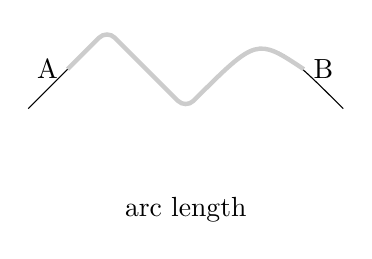
\begin{tikzpicture}
\title{Arc length}
 \draw [rounded corners] (0,0) -- (1,1) 
           -- (2,0) .. controls (3,1) .. (4,0); 
	\draw [rounded corners,gray!40!white, ultra thick] (0.5, 0.5) -- (1,1) 
           -- (2,0)..controls (2.9,0.9)..(3.5,0.5);
	\node [below=1cm, align=flush center] at (2,0){arc length};
\node[left] at (0.5, 0.5){A};
\node[right] at (3.5, 0.5){B};
\end{tikzpicture}
\begin{tikzpicture}
	\node[regular polygon, regular polygon sides=5, draw, inner sep=0.8cm, color = gray!40!white, ultra thick] at (0,0) {};
	\node [below=1.2cm, align=flush center] at (0,0){perimeter};
\end{tikzpicture}
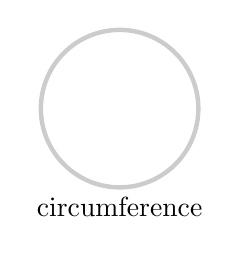
\begin{tikzpicture}
\draw [gray!40!white, ultra thick] (0,0)circle [radius = 1cm];
\node [below=1cm, align=flush center] at (0,0){circumference};
\end{tikzpicture}
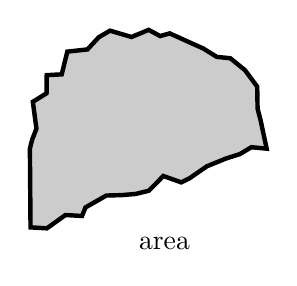
\begin{tikzpicture}
\draw [fill=gray!40!white,xshift=2cm, ultra thick,
decoration={random steps,segment length=2mm}]
decorate { (0,0) -- (3,1) arc (0:180:1.5)} -- cycle;
\node [below=1cm, align=flush center] at (3.7,1){area};
\end{tikzpicture}
\end{center}

\section{The circle}

\noindent Choose a point somewhere in the middle of a sheet of paper. We will call this point $m$ and refer to it as the "center" of the circle.  Draw a dot exactly 2 cm away from $m$. Draw another point also 2 cm away from $m$. And another. And another,... . If you draw all points that are a distance of 2 cm away from M you will have drawn something that looks like this:
\begin{center}
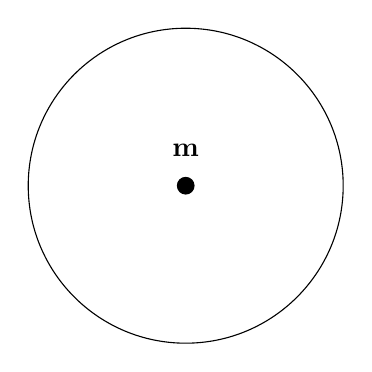
\begin{tikzpicture}
\draw (0,0)circle [radius = 2cm];
\filldraw (0,0) circle [radius = 3pt] node[above=2.5mm]{\textbf{m}};
\end{tikzpicture}
\end{center}
\noindent This is a \textbf{circle} of radius $2$ cm and center $m$. The \textbf{radius} of a circle is the distance from its center to any of its points. The \textbf{diameter} is the distance from any point of the circle to a point exactly opposite it. The line connecting such $2$ points passes through the center and has length $d = 2R$.
\begin{center}
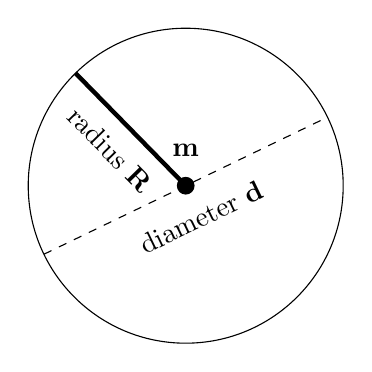
\begin{tikzpicture}
\draw (0,0) circle [radius = 2cm];
\filldraw (0,0) circle [radius = 3pt] node[above=2.5mm]{\textbf{m}};
\draw [ultra thick] (0,0) -- node[sloped, anchor=center,below=1mm]{radius $\bf{R}$}(-1.4,1.43);
\draw [dashed] (-1.8,-0.87) -- node[sloped, anchor=center,below=2mm]{diameter $\bf{d}$}(1.8,0.87);
\end{tikzpicture}
\end{center}
\noindent Though the circle is a seemingly simple geometric figure, it has several interesting and some non-intuitive properties. All circles, no matter how large or small, share the following property: \textbf{The circumference of the circle divided by its diameter is equal to $\pi$}. This is actually one of the multiple ways to define $\pi$:
\begin{equation}
\label{DefPi}
\frac{\textit{circumference of circle}}{\textit{diameter}} = \frac{\textit{circumference of circle}}{2 R} = \pi
\end{equation}
\noindent The number $\pi$ is often approximated by $3.14$, but as was mentioned in section \ref{RealNumbersSet}, $\pi$ is actually an irrational number and as such has an infinite non-repeating decimal tail. Multiplying both sides of equation (\ref{DefPi}) by $2R$ gives us the formula for the circumference $C$ of a circle:
\begin{equation}
\label{CircumCirc}
C = 2 \pi R
\end{equation}
A circle with radius $R$ can be shown to have area $A$ equal to\footnote{In chapter \ref{IntegralChapter} we will discuss techniques to prove this and similar formulas.}
\begin{equation}
A = \pi R^2
\end{equation}
\noindent One consequence of this is that if we draw a second circle with radius twice as large as the first one, its circumference will also be doubled but the area will be $4$ times larger (because of square in the formula for the area).

\section{Looking at it from a different angle}

\noindent Let us look at two (straight) lines $L_1$ and $L_2$. There are 3 possible cases:
\begin{center}
\begin{tikzpicture}
\draw (-2,-2) node [right=0.2cm]{$L_1$}-- (2,2);
\draw (-2,-2) node [left= 0.2cm]{$L_2$}-- (2,2);
%\draw (-3,0) node[above] {$L_2$} -- (2,1);
\end{tikzpicture}
\begin{tikzpicture}
\draw (-2,-2) node [below]{$L_1$}-- (2,2);
\draw (-3,0) node[above] {$L_2$} -- (2,1);
\end{tikzpicture}
\begin{tikzpicture}
\draw (-2,-2) node [right=0.2cm]{$L_1$}-- (2,2);
\draw (-2,-1) node[left=0.2cm] {$L_2$} -- (2,3);
\end{tikzpicture}
\end{center}
\begin{enumerate}
\item \textbf{Equal lines} are completely overlapping and thus have infinitely many points in common.
\item \textbf{Intersecting lines} have exactly $1$ point in common.
\item \textbf{Parallel lines} never touch and thus have no points in common. This is written as $L_1 \parallel L_2$.
\end{enumerate}
\noindent Whenever $2$ lines intersect, they form $4$ "openings" between them, known as \textbf{angles}.
\begin{center}
\begin{tikzpicture}[scale = 1.5]
\coordinate (A) at (-130:1.5);
\coordinate (B) at (0,0);
\coordinate (C) at (50:1.5);
\coordinate (D) at (-80:1.5);
\coordinate (E) at (100:1.5);
\draw [ultra thick] (A) -- (C);
\draw [ultra thick] (D) -- (E);
\draw[color=black, ultra thick] pic["$\alpha$", draw=gray!10!black, ultra thick, angle eccentricity=1.2, angle radius=1.3cm] {angle=A--B--D};
\draw pic["$\beta$", draw=gray!60!black, ultra thick, angle eccentricity=1.2, angle radius=0.8cm] {angle=D--B--C};
\draw pic["$\gamma$", draw=gray!30!black, ultra thick, angle eccentricity=1.2, angle radius=1.3cm] {angle=C--B--E};
\draw pic["$\delta$", draw=gray!80!black, ultra thick, angle eccentricity=1.2, angle radius=0.9cm] {angle=E--B--A};
\end{tikzpicture}
\end{center}
\noindent In \ref{Degr} and \ref{Radi} we will introduce two different units for angles. Afterwards, in \ref{AngRel} we will discuss some relations between angles, and we will show for example that it is sufficient to know $1$ one of the angles above, to know all of them.

\subsection{degrees}
\label{Degr}

\noindent For now, we focus on any of the angles formed by the $2$ lines and disregard the others. We take a horizontal line and consider the angle formed by rotating a second line around it. 
\begin{center}
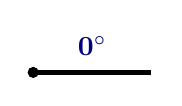
\begin{tikzpicture}[scale = 1.5]
\coordinate (A) at (1,0);
\coordinate (B) at (0,0);
\coordinate (C) at (0:1cm);
\filldraw[fill=blue!20!white, draw=blue!50!black] (0,0) -- (7mm,0mm)
	arc [start angle=0, end angle=0, radius=7mm, color=black] -- cycle;
\draw (A) -- (B) -- (C)[color=black, ultra thick];
\node [node font=\normalsize, color=blue!50!black] at (0.5,0.22) {$\bf{0^{\circ}}$};
\filldraw (B) circle [radius=1.2pt];
\end{tikzpicture}
\begin{tikzpicture}[scale = 1.5]
\coordinate (A) at (1,0);
\coordinate (B) at (0,0);
\coordinate (C) at (30:1cm);
\draw (A) -- (B) -- (C)[color=black, ultra thick] pic[draw=gray, ultra thick, ->, angle eccentricity=1.2, angle radius=7mm]
    {angle=A--B--C};
\node [node font=\normalsize, color=blue!50!black] at (0.9,0.22) {$\bf{30^{\circ}}$};
\end{tikzpicture}
\begin{tikzpicture}[scale = 1.5]
\coordinate (A) at (1,0);
\coordinate (B) at (0,0);
\coordinate (C) at (150:1cm);
\draw (A) -- (B) -- (C)[color=black, ultra thick]
	pic[draw=gray, ultra thick, ->, angle eccentricity=1.2, angle radius=7mm]
    {angle=A--B--C};
\node [node font=\normalsize, color=blue!50!black] at (0.2,0.7) {$\bf{150^{\circ}}$};
\end{tikzpicture}
\begin{tikzpicture}[scale = 1.5]
\coordinate (A) at (1,0);
\coordinate (B) at (0,0);
\coordinate (C) at (220:1cm);
\draw (A) -- (B) -- (C)[color=black, ultra thick]pic[draw=gray, ultra thick, ->, angle eccentricity=1.2, angle radius=7mm]
    {angle=A--B--C};
\node [node font=\normalsize, color=blue!50!black] at (0,0.7) {$\bf{220^{\circ}}$};
\end{tikzpicture}
\begin{tikzpicture}[scale = 1.5]
\coordinate (A) at (1,0);
\coordinate (B) at (0,0);
\coordinate (C) at (300:1cm);
\draw (A) -- (B) -- (C)[color=black, ultra thick]
	pic[draw=gray, ultra thick, ->, angle eccentricity=1.2, angle radius=7mm]
    {angle=A--B--C};
\node [node font=\normalsize, color=blue!50!black] at (0,0.7) {$\bf{300^{\circ}}$};
\end{tikzpicture}
\begin{tikzpicture}[scale = 1.5]
\coordinate (A) at (1,0);
\coordinate (B) at (0,0);
\coordinate (C) at (359.9:1cm);
\draw (A) -- (B) -- (C)[color=black, ultra thick]
	pic[draw=gray, ultra thick, ->, angle eccentricity=1.2, angle radius=7mm]
    {angle=A--B--C};
\node [node font=\normalsize, color=blue!50!black] at (0,0.9) {$\bf{360^{\circ}}$};
\end{tikzpicture}
\end{center}
\noindent One common unit for angles is known as \textbf{degrees} denoted by the symbol $\bf{^\circ}$. When the lines are overlapping (or simply parallel) the angle is said to be a $0^{\circ}$ angle. A full rotation\footnote{The historical reason for dividing the circle into $360^{\circ}$ is not exactly known. One often-stated hypothesis is that this is part of the legacy of the Babylonian sexagecimal numeral system (base 60) that also gave us the division of an hour into 60 minutes and a minute into 60 seconds.} corresponds to $360^{\circ}$. Therefore an angle of $0^{\circ}$ and one of $360^{\circ}$ are equal.\\

\noindent We emphasize that there is no logical reason why a circle has to be divided into exactly $360$ equal parts. Below is a circle divided into $10$ equal parts. We could have called the angle of each of these parts a zorm and circles would therefore be constituted of $10$ zorms. For historical reasons though the convention is to divide circles into $360$ equal slices where the angle of one such slice is called one degree.

\begin{center}
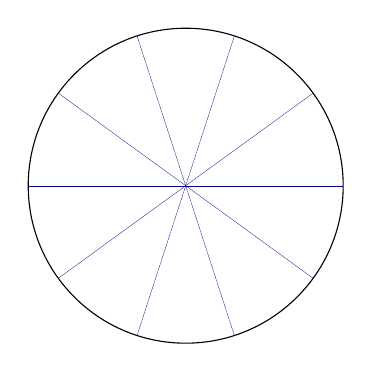
\begin{tikzpicture}
\draw (0,0) circle [radius = 2];
\foreach \ang in {0,36,...,360}{
	\draw [color=blue!50!black ,ultra thin] (0,0) -- (\ang:2);
	}
\end{tikzpicture}
\begin{tikzpicture}[scale=1.3]
\draw [ultra thick] (0,0) -- (60:1.9);
\draw [ultra thick] (0,0) -- (290:1.9);
\coordinate (A) at (0:2);
\coordinate (B) at (0,0);
\coordinate (C) at (60:1.3cm);
\coordinate (D) at (290:1cm);
\coordinate (E) at (-70:0.7cm);
\draw [ultra thick] (0,0) -- (2.2,0);
\draw pic["$\bf{60^{\circ}}$",draw=black, ultra thick, ->, angle eccentricity=1.5, angle radius=1.5cm] {angle=A--B--C};
\draw pic["$\bf{290^{\circ}}$",draw=black, ultra thick, ->, angle eccentricity=1.5, angle radius=0.7cm] {angle=A--B--D};
\draw pic["$\bf{-70^{\circ}}$",draw=gray!70!black, ultra thick, <-, angle eccentricity=1.5, angle radius=1cm] {angle=E--B--A};
\end{tikzpicture}
\end{center}
\noindent By convention, angles are positive if they are counterclockwise and negative if they are clockwise (also here, there is no logic to this, it is simply a historical convention). The absolute value of the angle tells us how large the opening between the $2$ lines is. Its sign tells us whether the opening is to be considered clockwise (negative) or counterclockwise (positive). As you can see on the figure the same two lines form both the angle of $290^{\circ}$ and that of $-70^{\circ}$. The difference is only whether we consider the opening to be read clockwise or counterclockwise.\\

\noindent Angles can also have absolute value larger than $360^{\circ}$. For instance, $420^{\circ}$ is a full circle plus an opening of $60^{\circ}$.
\begin{center}
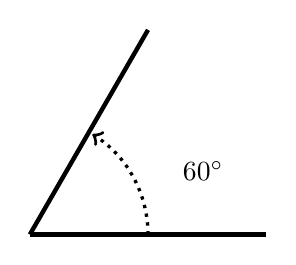
\begin{tikzpicture}
 \draw [ultra thick] ( 0,0) -- (3,0);
 \draw [ultra thick] (0,0) -- (60:3); 
%\draw [dashed, black,->] () arc (); 

\draw [->,very thick, dotted] (1.5,0) arc [start angle=0, end angle=58, radius=1.5];

%(1.5,0) arc[start angle=0, end angle = 60,  radius = 1.5,->] (60:1.5);
\node[black] at (2.2, 0.8) {$60^{\circ}$};
 \bigangle[gray,dashed]{420};
\end{tikzpicture}
\end{center}
\noindent These angles represent the same opening between the two lines. The grey one is just thought of as having made a full circle prior to ending up at the same place as the line of the $60^{\circ}$ angle.\\

\noindent When $2$ lines form an angle of $90^{\circ}$ the angle is called a \textbf{right} angle and the lines are said to be \textbf{perpendicular}, written as $L_1 \perp L_2$. Right angles are marked in figures in the following manner: 
\begin{center}
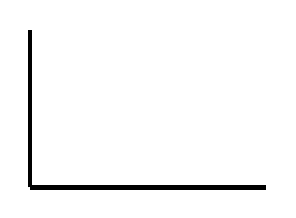
\begin{tikzpicture}
\coordinate (A) at (3, 0) {};
        \coordinate (B) at (0, 0) {};
        \coordinate (C) at (0, 2) {};
\tkzMarkRightAngle[size=.7](A,B,C);
\tkzLabelAngle[dist=.5](A,B,C){};
 \draw [ultra thick] (B) -- (A);
 \draw [ultra thick] (B) -- (C); 
\end{tikzpicture}
\end{center}

\subsection{Radians}
\label{Radi}

\noindent What is the relation between an angle $\alpha$ and the size of the arc length $L$ formed by it?
\begin{center}
\begin{tikzpicture}[scale= 2.2]
\draw [dashed, gray] (0,0) circle [radius = 1];
\coordinate (A) at (-30:1);
\coordinate (B) at (0,0);
\coordinate (C) at (45:1);
\draw [black!50!brown,thin] (B) -- node[sloped, anchor=center,below=2mm]{$R$}(A);
\draw [black!50!brown, thin] (B) -- (C);
\draw pic["$\bf{\alpha}$",draw=blue!80!black, dashed, angle eccentricity=1.3, angle radius=1.3cm] {angle=A--B--C};
\draw pic["$\bf{L}$",draw=blue!50!black, ultra thick, angle eccentricity=1.2, angle radius=2.2cm] {angle=A--B--C};
\end{tikzpicture}
\end{center}
\noindent Equation (\ref{CircumCirc}) tells us that if $\alpha=360^{\circ}$ then $L=2\pi R$, the circumference of the circle. If we choose angle $\alpha=180^{\circ}$, corresponding to half the angle of a full circle, the arc length $L$ would be half the circumference of the full circle: $L=\frac{2 \pi R}{2} = \pi R$. An angle of $90^{\circ}$, which is a quarter circle, creates an arc length of a quarter of the circumference of the circle: $L = \frac{2 \pi R}{4} = \frac{\pi R}{2}$. This reasoning holds for any angle. For instance, an angle $\alpha = 36^{\circ}$ corresponding to one tenth of a full circle (i.e. $\frac{36}{360} = \frac{1}{10}$) covers an arc length of one tenth of the circumference: $L = \frac{2 \pi R}{10} = \frac{\pi R}{5}$.\\

\noindent As mentioned earlier, the choice of dividing the circle into $360$ equal parts and calling the size of each a degree is an arbitrary choice made by accidents of history. Instead of dividing the circle into $360$ equal parts, we divide it into $2\pi$ parts (which is approximately $2\times 3.14 = 6.28$) and we call each part a \textbf{radian}. A full circle corresponds therefore to an angle of $2 \pi$ radians, half a circle to $\pi$ radians and so forth. The advantage of this unit is that it explicitly relates the size of the angle with the length of the arc length it forms: an angle of size $\alpha$ radians, in a circle of radius $R$ forms an arc length equal to
\begin{equation}
\label{WrongRadians}
L = R \alpha
\end{equation}
\noindent Can we see that easily? Take for instance $\alpha = 2\pi$ (a full circle), than the arc length is according to (\ref{WrongRadians}) equal to $L = R 2 \pi $, which is indeed the circumference of the circle. Or if we take $\alpha=\frac{\pi}{2}$ (a quarter of a circle), the arc length is $L = R \frac{\pi}{2} = \frac{2 \pi R}{4}$ which is indeed the arc length of a quarter of a circle. Keep the following in mind when working with radians:
\begin{enumerate}
\item The unit radian is often abbreviated as rad. But it is actually more common to omit it altogether and speak about an angle of for instance $\frac{\pi}{4}$ instead of $\frac{\pi}{4}$ rad. This is only done with radians, not with degrees.
\item A negative arc length or a negative radius is meaningless. Lengths are always positive. But angles can be negative and so negative radians do make sense. Remember, a negative angle simply means that it is considered clockwise. Equation (\ref{WrongRadians}) is therefore wrong for negative angles. A correcter version is 
\begin{equation}
L = R |\alpha|
\end{equation}
\item Whenever $\alpha$ is larger than $2\pi$, the arc length $L$ is to be understood as the arc length of the angle plus however many times a full circle is covered. For instance, an angle of $5 \pi$ radians corresponds to $2$ full circumferences ($ 2 \times 2 \pi R$) plus half a circumference ($\frac{2 \pi R}{2}$) which gives a total arc length of $ 2 \times 2 \pi R + \frac{2 \pi R}{2} = 4 \pi R + \frac{2 \pi R}{2} = 5 \pi R$. 
\end{enumerate}
\noindent Degrees and radians are simply different units for the same quantity: angles. Below is a table with corresponding values in both units.\\
\begin{center}
\begin{tabular}{ |c|c|c| }
  \hline
  Figure & Degrees & Radians\\
  \hline
	& & \\
  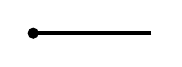
\begin{tikzpicture}[scale = 1.5]
\coordinate (A) at (1,0);
\coordinate (B) at (0,0);
\coordinate (C) at (0:1cm);
\filldraw[fill=blue!20!white, draw=blue!50!black] (0,0) -- (7mm,0mm)
	arc [start angle=0, end angle=0, radius=7mm] -- cycle;
\draw (A) -- (B) -- (C)[color=black, ultra thick];
\filldraw (B) circle [radius=1.2pt];
\end{tikzpicture} & $0$ & $0$\\& & \\
\hline
& & \\
	\begin{tikzpicture}[scale = 1.5]
\coordinate (A) at (1,0);
\coordinate (B) at (0,0);
\coordinate (C) at (30:1cm);
\draw (A) -- (B) -- (C)[color=black, ultra thick] pic[draw=gray!50!white, ultra thick, ->, angle eccentricity=1.2, angle radius=7mm]
    {angle=A--B--C};
\end{tikzpicture} & $30$ & $ \pi / 6$\\& & \\
	\hline
	& & \\
		\begin{tikzpicture}[scale = 1.5]
\coordinate (A) at (1,0);
\coordinate (B) at (0,0);
\coordinate (C) at (45:1cm);
\draw (A) -- (B) -- (C)[color=black, ultra thick] pic[draw=gray!50!white, ultra thick, ->, angle eccentricity=1.2, angle radius=7mm]
    {angle=A--B--C};
\end{tikzpicture} & $45$ & $\pi/4$\\& & \\
	\hline
	& & \\
	\begin{tikzpicture}[scale = 1.5]
\coordinate (A) at (1,0);
\coordinate (B) at (0,0);
\coordinate (C) at (60:1cm);
\draw (A) -- (B) -- (C)[color=black, ultra thick] pic[draw=gray!50!white, ultra thick, ->, angle eccentricity=1.2, angle radius=7mm]
    {angle=A--B--C};
\end{tikzpicture} & $60$ & $\pi/3$\\& & \\
	\hline
	& & \\
	\begin{tikzpicture}[scale = 1.5]
\coordinate (A) at (1,0);
\coordinate (B) at (0,0);
\coordinate (C) at (90:1cm);
\draw (A) -- (B) -- (C)[color=black, ultra thick] pic[draw=gray!50!white, ultra thick, ->, angle eccentricity=1.2, angle radius=7mm]
    {angle=A--B--C};
\end{tikzpicture} & $90$ & $\pi/2$\\& & \\
	\hline
	& & \\
	\begin{tikzpicture}[scale = 1.5]
\coordinate (A) at (1,0);
\coordinate (B) at (0,0);
\coordinate (C) at (180:1cm);
\draw (A) -- (B) -- (C)[color=black, ultra thick] pic[draw=gray!50!white, ultra thick, ->, angle eccentricity=1.2, angle radius=7mm]
    {angle=A--B--C};
		\filldraw (B) circle [radius=1.2pt];
\end{tikzpicture} & $180$ & $\pi$\\& & \\
	\hline
	& & \\
		\begin{tikzpicture}[scale = 1.5]
\coordinate (A) at (1,0);
\coordinate (B) at (0,0);
\coordinate (C) at (359.9:1cm);
\draw (A) -- (B) -- (C)[color=black, ultra thick] pic[draw=gray!50!white, ultra thick, ->, angle eccentricity=1.2, angle radius=7mm]
    {angle=A--B--C};
		\filldraw (B) circle [radius=1.2pt];
\end{tikzpicture} & $360$ & $2 \pi$\\& & \\
	\hline
\end{tabular}
\end{center}
\noindent A full circle corresponds to either $360^{\circ}$ or to $2\pi$ radians:
\begin{eqnarray*}
 & 2 \pi \text{ rad} =  360^{\circ} &  \\
\Leftrightarrow & 1 \text{ rad} =  \frac{360^{\circ}}{2\pi}  & \left( \text{divide both sides by }2\pi \right) \\
\Leftrightarrow & 1 \text{ rad} = \frac{180^{\circ}}{\pi} & \\
\Leftrightarrow & x \text{ rad} = x \frac{180^{\circ}}{\pi} & \left( \text{multiply both sides with }x \right)\\
\end{eqnarray*}
\noindent From this we conclude that an angle of size $x$ when expressed in radians corresponds to an angle of $x\frac{180}{\pi}$ in degrees. The inverse relation is found by multiplying both sides by $\frac{\pi}{180}$:
\begin{eqnarray*}
x^{\circ} = x\frac{\pi}{180} \text{rad}
\end{eqnarray*}
\noindent In many math and physics texts radians are used rather than degrees. Unless explicitly stated by using the ${\circ}$ symbol, we will always work in radians throughout the text.

\subsection{Angular relations}
\label{AngRel}

\noindent Now that we have a vocabulary for discussing angles we derive some common relations between them.
\begin{center}
\begin{tikzpicture}[scale = 1.5]
\coordinate (A) at (1,0);
\coordinate (B) at (0,0);
\coordinate (C) at (180:1cm);
\draw (A) -- (B) -- (C)[color=black, ultra thick] pic["$180^{\circ}$",draw=gray!50!white, ultra thick, angle eccentricity=1.5, angle radius=7mm]
    {angle=A--B--C};
		\filldraw (B) circle [radius=1.2pt];
\end{tikzpicture}
\begin{tikzpicture}[scale = 1.5]
\coordinate (A) at (1.2,0);
\coordinate (B) at (0,0);
\coordinate (C) at (180:1.2cm);
\coordinate (D) at (30:1.2cm);
\coordinate (E) at (145:1.2cm);
\coordinate (F) at (-1.2,0);
\draw (A) -- (B) -- (D)[color=black, ultra thick] pic["$\alpha$", draw=gray!20!white, ultra thick, angle eccentricity=1.2, angle radius=1.2cm]
    {angle=A--B--D};
\draw (D) -- (B) -- (F)[color=black, ultra thick] pic["$\beta$", draw=gray!80!white, ultra thick, angle eccentricity=1.2, angle radius=0.8cm]
    {angle=D--B--F};
\end{tikzpicture}
\begin{tikzpicture}[scale = 1.5]
\coordinate (A) at (1.2,0);
\coordinate (B) at (0,0);
\coordinate (C) at (180:1.2cm);
\coordinate (D) at (30:1.2cm);
\coordinate (E) at (145:1.2cm);
\coordinate (F) at (-1.2,0);
\draw (A) -- (B) -- (D)[color=black, ultra thick] pic["$\gamma$", draw=gray!10!white, ultra thick, angle eccentricity=1.2, angle radius=1.3cm]
    {angle=A--B--D};
\draw (D) -- (B) -- (E)[color=black, ultra thick] pic["$\delta$", draw=gray!50!white, ultra thick, angle eccentricity=1.3, angle radius=7mm]
    {angle=D--B--E};
\draw (E) -- (B) -- (F)[color=black, ultra thick] pic["$\epsilon$", draw=gray!90!white, ultra thick, angle eccentricity=1.2, angle radius=1.3cm]
    {angle=E--B--F};
\end{tikzpicture}
\end{center}
\noindent A straight line corresponds to an angle of $180^{\circ}$. Consequently, angles that form together a straight line add up to $180^{\circ}$. This means that
\begin{eqnarray*}
 \alpha + \beta  & = 180^{\circ} \\
\gamma + \delta + \epsilon & = 180^{\circ} 
\end{eqnarray*}
\noindent Two angles are called supplementary whenever they sum up to $180^{\circ}$. In the figures above, $\alpha$ and $\beta$ are supplementary.\\

\noindent Let us go back to the $4$ angles formed by $2$ intersecting lines from the beginning of this section.
\begin{center}
\begin{tikzpicture}[scale = 1.5]
\coordinate (A) at (-130:1.5);
\coordinate (B) at (0,0);
\coordinate (C) at (50:1.5);
\coordinate (D) at (-80:1.5);
\coordinate (E) at (100:1.5);
\draw [ultra thick] (A) -- (C);
\draw [ultra thick] (D) -- (E);
\draw[color=black, ultra thick] pic["$\alpha$", draw=gray!10!white, ultra thick, angle eccentricity=1.2, angle radius=1.3cm] {angle=A--B--D};
\draw pic["$\beta$", draw=gray!30!white, ultra thick, angle eccentricity=1.2, angle radius=0.8cm] {angle=D--B--C};
\draw pic["$\gamma$", draw=gray!50!white, ultra thick, angle eccentricity=1.2, angle radius=1.3cm] {angle=C--B--E};
\draw pic["$\delta$", draw=gray!50!white, ultra thick, angle eccentricity=1.2, angle radius=0.9cm] {angle=E--B--A};
\end{tikzpicture}
\end{center}
\noindent A first claim is that all pairs of adjacent angles are supplementary. This simply follows from the fact that each adjacent pair forms a straight line.
$$
\alpha + \beta = \beta + \gamma = \gamma + \delta = \delta + \alpha = 180^{\circ} 
$$
\noindent A second relation is that opposing angles are equal: $\alpha =\gamma$ and $\beta = \delta$. This is a direct consequence of the first property:
\begin{eqnarray*}
& \alpha + \delta  = 180^{\circ} = \gamma + \delta \\
\Rightarrow & \alpha + \delta = \gamma + \delta \\
\Leftrightarrow & \alpha = \gamma
\end{eqnarray*}
\noindent The last equality was gotten by deducting $\delta$ from both sides of the equation above (which we learned in chapter \ref{Chap_Func} is allowed). By the same logic it can be shown that $\beta = \delta$. We thus found that opposing angles are equal.\\

\noindent A consequence of these properties is that if any of the $4$ angles is a right angle, than they are all right angles. Take for instance $\delta = 90^{\circ}$. From the first property it follows that both $\alpha$ and $\gamma$ are right. And from the second property it follows that $\beta$ is also right.\\

\noindent For a final angular relation, we start with $2$ intersecting lines. We translate one of the lines, keeping it parallel to its previous position\footnote{A translation is a displacement in which no rotation takes place.}. As can be seen on the figure below, such a translation leaves the angle unchanged.
\begin{center}
\begin{tikzpicture}[baseline=(current bounding box.center),scale=0.8]
\coordinate (A) at (0,0); %Not used
\coordinate (B) at (-2,-2);% L1 left
\coordinate (C) at (2,2); % L1 right
\coordinate (D) at (-2,-1);% L2 left
\coordinate (E) at (2,3); %L2 right
\coordinate (F) at (-2,0.5); %L3 left
\coordinate (G) at (2,1); % L3 right
\coordinate (H) at (0.857142857142857,0.857142857142857); % L1 crosses L3
\coordinate (I) at (-0.285714285714286,0.714285714285714); % L2 crosses L3
\draw [thick] (D) -- (E)node[right]{$L_1$};
\draw [thick] (F)node[left]{$L_3$} -- (G);
\draw[color=black, ultra thick] pic["$\alpha$", draw=black, ultra thick, angle eccentricity=1.4, angle radius=0.4cm] {angle=E--I--F};
%\tkzMarkAngle[size=0.4](E,I,F);
\end{tikzpicture}
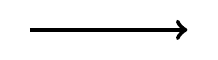
\begin{tikzpicture}[baseline=(current bounding box.center)]
\draw[->, ultra thick] (-1,0) -- (1,0);
\end{tikzpicture}
\begin{tikzpicture}[baseline=(current bounding box.center)]
\coordinate (A) at (0,0); %Not used
\coordinate (B) at (-1,-1);% L1 left
\coordinate (C) at (3,3); % L1 right
\coordinate (D) at (-2,-1);
\coordinate (E) at (2,3);
\coordinate (F) at (-2,0.5); %L3 left
\coordinate (G) at (2,1); % L3 right
\coordinate (H) at (0.857142857142857,0.857142857142857); % L1 crosses L3
\coordinate (I) at (-0.285714285714286,0.714285714285714); % L2 crosses L3
\draw [dashed] (D) -- (E)node[right]{};
\draw [thick] (B) -- (C)node[right]{$L_1$};
\draw [thick] (F)node[left]{$L_3$} -- (G);
\draw[color=black] pic["$\alpha$", draw=black, ultra thick, angle eccentricity=1.4, angle radius=0.4cm] {angle=E--I--F};
\draw[color=black, ultra thick] pic["$\alpha$", draw=black, ultra thick, angle eccentricity=1.4, angle radius=0.4cm] {angle=C--H--F};
\draw[->, dashed, thick, shorten <=5pt, shorten >=5pt](E) -- (C){};
\end{tikzpicture}
\end{center}
From this it follows that the corresponding angles of $2$ parallel lines ($L_1$ and $L_2$) intersected by a third line ($L_3$) are equal. 
\begin{center}
\begin{tikzpicture}[scale = 1.2]
\coordinate (A) at (0,0); %Not used
\coordinate (B) at (-2,-2);% L1 left
\coordinate (C) at (2,2); % L1 right
\coordinate (D) at (-2,-1);% L2 left
\coordinate (E) at (2,3); %L2 right
\coordinate (F) at (-2,0.5); %L3 left
\coordinate (G) at (2,1); % L3 right
\coordinate (H) at (0.857142857142857,0.857142857142857); % L1 crosses L3
\coordinate (I) at (-0.285714285714286,0.714285714285714); % L2 crosses L3
\draw [thick] (B) -- (C)node[right]{$L_1$};
\draw [thick] (D) -- (E)node[right]{$L_2$};
\draw [thick] (F)node[left]{$L_3$} -- (G);
\draw[color=black, ultra thick] pic["$\alpha$", draw=black, ultra thick, angle eccentricity=1.4, angle radius=0.4cm] {angle=E--I--F};
\draw[color=black, ultra thick] pic["$\beta$", draw=black, ultra thick, angle eccentricity=1.3, angle radius=0.8cm] {angle=F--I--D};
\draw[color=black, ultra thick] pic["$\gamma$", draw=black, ultra thick, angle eccentricity=1.7, angle radius=0.3cm] {angle=D--I--G};
\draw[color=black, ultra thick] pic["$\delta$", draw=black, ultra thick, angle eccentricity=1.4, angle radius=0.5cm] {angle=G--I--E};
\draw[color=black, ultra thick] pic["$\epsilon$", draw=black, ultra thick, angle eccentricity=1.4, angle radius=0.4cm] {angle=C--H--F};
\draw[color=black, ultra thick] pic["$\zeta$", draw=black, ultra thick, angle eccentricity=1.4, angle radius=0.6cm] {angle=F--H--B};
\draw[color=black, ultra thick] pic["$\eta$", draw=black, ultra thick, angle eccentricity=1.8, angle radius=0.3cm] {angle=B--H--G};
\draw[color=black, ultra thick] pic["$\theta$", draw=black, ultra thick, angle eccentricity=1.4, angle radius=0.5cm] {angle=G--H--C};
\end{tikzpicture}
\end{center}
\noindent In the figure above, the angles are therefore related in the following way.
\begin{eqnarray*}
\alpha = \gamma = \epsilon = \eta \\
\beta = \delta = \zeta = \theta \\
\alpha = 180^{\circ} - \beta
\end{eqnarray*}

\noindent To summarize, the properties of angles we discussed are:
\begin{itemize}
\item Adjacent angles are supplementary
\item Opposing angles are equal
\item A straight line intersecting $2$ parallel lines creates $8$ angles. Equivalent angles are equal.
\end{itemize}

\section{The shape of things}

\noindent We already introduced the circle and some of its properties. In this section we will be looking at some other two-dimensional shapes: triangles, rectangles and squares. What we are mainly interested in are general statements, meaning that they are true for a large class of shapes. The fact that the circumference of a circle divided by its diameter is equal to $\pi$ is true for any circle, no matter how small or large. If it were only true for one specific circle it would be much less interesting or useful. The power of statements in mathematics depends on how generally valid they are.

\subsection{Triangles}
\label{Intro_Triangles}

\noindent A triangle is a closed flat shape with 3 angles (duh...). Though it may not seem obvious at first, the study of triangles and their properties brings us a very long way towards knowing enough math to actually do physics.\\

\noindent The first property of interest is that the sum of the internal angles of any triangle equals $180^{\circ}$ (i.e. $\pi$ radians). To prove this, we consider an arbitrary triangle.
\begin{center}
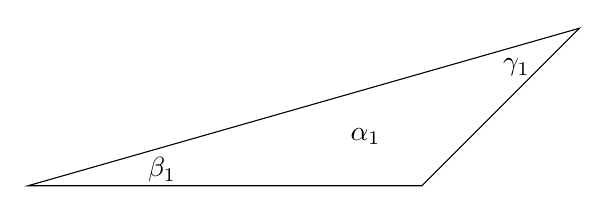
\begin{tikzpicture}
\coordinate (A) at (-3,0);
\coordinate (B) at (2,0);
\coordinate (C) at (4,2);
\draw[color=black] (A) -- (B) -- (C) -- cycle;
\tkzMarkAngle[size=0.5](C,B,A){};%alpha_1
\tkzMarkAngle[size=0.7](A,C,B){};%gamma_1
\tkzMarkAngle[size=1.2](B,A,C){};%beta_1
\node at (-1.3,0.2){$\beta_1$};
\node at (3.2,1.5){$\gamma_1$};
\node at (B)[above left=4mm]{$\alpha_1$};
\end{tikzpicture}
\end{center}
\noindent The quantity we are interested in is the sum of the angles: $\alpha_1+\beta_1+\gamma_1$. Let us first draw a line parallel to one of the sides of the triangle. For instance a (horizontal) line parallel to the bottom of triangle, which we draw touching the triangle at its highest point. We also extend both other sides of the triangle (the dashed lines), so that these intersect the new horizontal line.
\begin{center}
\begin{tikzpicture}
\coordinate (A) at (-3,0);
\coordinate (B) at (2,0);
\coordinate (C) at (4,2);
\coordinate (D) at (7,2.85714285714286); % y = (2/7)x +(6/7) (line BC)
\coordinate (E) at (7,5); % y = x - 2 (line AC)
\coordinate (F) at (-3.5,2);
\coordinate (G) at (7,2);
\draw[color=black] (A) -- (B) -- (C) -- cycle;
\tkzMarkAngle[size=0.5](C,B,A){};%alpha_1
\tkzMarkAngle[size=0.7](A,C,B){};%gamma_1
\tkzMarkAngle[size=1.2](B,A,C){};%beta_1
\node at (-1.3,0.2){$\beta_1$};
\node at (3.2,1.5){$\gamma_1$};
\node at (B)[above left=4mm]{$\alpha_1$};
\draw[thin, dashed] (C) -- (D);
\draw[thin, dashed] (C) -- (E);
\draw (F) -- (G);
\tkzMarkAngle[size=0.5](E,C,F){};%alpha_2
\tkzMarkAngle[size=1.5](D,C,E){};%gamma_2
\tkzMarkAngle[size=1.7](G,C,D){};%beta_2
\node at (6,2.3){$\beta_2$};
\node at (5.7,3){$\gamma_2$};
\node at (3.7,2.7){$\alpha_2$};
\end{tikzpicture}
\end{center}
\noindent Because angles $\gamma_1$ and $\gamma_2$ are opposing angles, they are equal. As the bottom side of the triangle is parallel to the horizontal line we added above it, and the dashed lines are the extensions of the $2$ other sides, it follows that $\alpha1$ and $\alpha_2$ are corresponding angles, and so are $\beta_1$ and $\beta_2$. We know that $\alpha_2 + \beta_2 + \gamma_2 = 180^{\circ}$ because they form a straight line. Which finally leads to $\alpha_1 + \beta_1 + \gamma_1 = 180^{\circ}$.\\

\noindent The argument given does not depend on any specific property of this triangle. It would work as well for any other triangle. Nor would it fail if we had chosen to draw a line parallel to either of the other sides. It seems that the angles of any triangle always\footnote{This is true in what is known as Euclidean geometry. When we extend the study of triangles to curved spaces, as is for instance the case in the context of the general theory of relativity, this result does not hold anymore.} add up to $180^{\circ}$.

\subsection{Rectangles and squares} 

\noindent We now switch to closed, flat shapes with $4$ angles, known as quadrilaterals or quadrangles. We will limit our discussion to a specific class of quadrangles known as \textbf{rectangles}. Their defining property is that they have $4$ right angles.
\begin{center}
\begin{tikzpicture}
\tkzDefPoint(-1,-1){A}
\tkzDefPoint(-1,1){B}
\tkzDefPoint(3,1){C}
\tkzDefPoint(3,-1){D};
\node at (-1,0)[left=3pt]{$W$};
\node at (1,-1)[below=3pt]{$L$};
\draw (A) node[below]{a}-- (B)node[above]{b} -- (C)node[above]{c} -- (D) node[below]{d} -- cycle;
\tkzMarkSegment[color=black, pos=.5, mark=||](B,C)
\tkzMarkSegment[color=black,pos=0.5,mark=||](A,D)
\tkzMarkSegment[color=black, pos=.5, mark=s|](A,B);
\tkzMarkSegment[color=black,pos=.5,mark=s|](D,C);
\tkzMarkRightAngle[size=.2, ultra thin](D,A,B);
\tkzMarkRightAngle[size=.2, ultra thin](A,B,C);
\tkzMarkRightAngle[size=.2, ultra thin](B,C,D);
\tkzMarkRightAngle[size=.2, ultra thin](C,D,A);
\end{tikzpicture}
\begin{tikzpicture}
\tkzDefPoint(-1,-1){A}
\tkzDefPoint(-1,1){B}
\tkzDefPoint(3,1){C}
\tkzDefPoint(3,-1){D};
\node at (3,0)[right=3pt]{$W$};
\node at (1,-1)[below=3pt]{$L$};
\draw (A) node[below]{a}-- (B)node[above]{b} -- (C)node[above]{c} -- (D) node[below]{d} -- cycle;
\draw (B) -- (D);
\tkzMarkSegment[color=black, pos=.5, mark=||](B,C)
\tkzMarkSegment[color=black,pos=0.5,mark=||](A,D)
\tkzMarkSegment[color=black, pos=.5, mark=s|](A,B);
\tkzMarkSegment[color=black,pos=.5,mark=s|](D,C);
\tkzMarkRightAngle[size=.2, ultra thin](D,A,B);
\tkzMarkRightAngle[size=.2, ultra thin](A,B,C);
\tkzMarkRightAngle[size=.2, ultra thin](B,C,D);
\tkzMarkRightAngle[size=.2, ultra thin](C,D,A);
\end{tikzpicture}
\end{center}
\noindent The lengths $ab$ ($=cd$) and $ad$ ($=bc$) are called the width $W$ and length $L$ of the rectangle, respectively. The tick marks in the middle of each of the sides are there to emphasize the equality of these sides: the same tick mark means they have the same length. The four angles are right angles, meaning that their sum is $360^{\circ}$. This can also be seen by drawing one of the diagonals of the rectangle. Any rectangle can be divided this way into $2$ triangles. As the angles of each of these sums up to $180^{\circ}$, the rectangle indeed has a total angle of $360^{\circ}$. Though we focus on rectangles, the argument and the conclusion that the angles add up to $360^{\circ}$ holds for any quadrangle.\\

\noindent The perimeter and area of a rectangle can be seen on the figure above to be
\begin{eqnarray*}
P = 2 L + 2 W \\
A = L \times W
\end{eqnarray*}
\noindent A \textbf{square} is a rectangle whose width and length are equal (i.e. its $4$ sides have an equal length). Squares are therefore a subclass of rectangles. 
\begin{center}
\begin{tikzpicture}
\tkzDefPoint(-1,-1){A}
\tkzDefPoint(-1,1){B}
\tkzDefPoint(1,1){C}
\tkzDefPoint(1,-1){D};
\node at (0,-1)[below=3pt]{$L$};
\draw (A) -- (B) -- (C) -- (D) -- cycle;
\tkzMarkSegment[color=black, pos=.5, mark=|](A,B)
\tkzMarkSegment[color=black, pos=.5, mark=|](B,C)
\tkzMarkSegment[color=black, pos=.5, mark=|](C,D)
\tkzMarkSegment[color=black, pos=.5, mark=|](D,A)
\tkzMarkRightAngle[size=.2, ultra thin](D,A,B);
\tkzMarkRightAngle[size=.2, ultra thin](A,B,C);
\tkzMarkRightAngle[size=.2, ultra thin](B,C,D);
\tkzMarkRightAngle[size=.2, ultra thin](C,D,A);
\end{tikzpicture}
\end{center}
\noindent A square with side $l$ has a perimeter and an area given by
\begin{eqnarray*}
P = 4 L \\
A = L^2
\end{eqnarray*}
\noindent which are just special cases of the rectangle formulas above with $L=W$.

\subsection{Pythagoras works when it's right}

\noindent The discussion in section (\ref{Intro_Triangles}) holds for all triangles. We now look at a specific kind of triangle known as a \textbf{right triangle}. These are defined as triangles that have a right angle\footnote{Triangles can never have more than $1$ right angle. Can you think of a reason for this?}.
\begin{center}
\begin{tikzpicture}[scale = 0.7]
\tkzDefPoint(0,0){A}
\tkzDefPoint(0,2){B}
\tkzDefPoint(5,0){C}
\node at (2.5,0)[below=3pt]{$C$};
\node at (0,1)[left=3pt]{$B$};
\node at (2.5,1)[above=3pt]{$A$};
\draw (A) -- (B) -- (C) -- cycle;
\tkzMarkRightAngle[size=.5, ultra thin](C,A,B);% alpha
\tkzMarkAngle[size=1.3](B,C,A){}; %beta
\tkzMarkAngle[size=0.5](A,B,C){}; % gamma
\node at (0.75,0.7){$\alpha$};
\node at (3.2,0.3){$\beta$};
\node at (0.5,1.2){$\gamma$};
\end{tikzpicture}
\end{center}
\noindent The sides of right triangles are always related by a relation known as the Pythagorean theorem:
$$
A^2 = B^2 + C^2
$$
\noindent where $A$ is the side of the triangle opposite the right angle (the initiated call it the hypotenuse, but who cares about a name?).\\

\noindent There are many different ways of proving the theorem. One elegant way is to take $4$ copies of the right triangle above and arrange them in the following ways:
\begin{center}
\begin{tikzpicture}[scale = 0.7]
\tkzDefPoint(0,0){A}
\tkzDefPoint(5,0){B}
\tkzDefPoint(7,0){C}
\tkzDefPoint(0,2){D};
\tkzDefPoint(7,5){E};
\tkzDefPoint(0,7){F};
\tkzDefPoint(2,7){G};
\tkzDefPoint(7,7){H};
\filldraw[color=black!20!gray] (A) -- (B) -- (D) -- cycle;
\filldraw[color=black!80!gray] (B) -- (C) -- (E) -- cycle;
\filldraw[color=black!60!gray] (D) -- (F) -- (G) -- cycle;
\filldraw[color=black!40!gray] (G) -- (H) -- (E) -- cycle;
\node at (2.5,1)[above=3pt]{$A$};
\node at (1,4.5)[right=3pt]{$A$};
\node at (6,2.5)[left=3pt]{$A$};
\node at (4.5,6)[below=3pt]{$A$};
\node at (0,1)[left=3pt]{$B$};
\node at (6,0)[below=3pt]{$B$};
\node at (7,6)[right=3pt]{$B$};
\node at (1,7)[above=3pt]{$B$};
\node at (2.5,0)[below=3pt]{$C$};
\node at (0,4.5)[left=3pt]{$C$};
\node at (7,2.5)[right=3pt]{$C$};
\node at (4.5,7)[above=3pt]{$C$};
\draw[thin](A) rectangle (H);
\node at (3.5,3.5){$A^2$};
\tkzMarkRightAngle[size=.5, ultra thin](E,B,D);
\tkzMarkRightAngle[size=.5, ultra thin](B,D,G);
\tkzMarkRightAngle[size=.5, ultra thin](D,G,E);
\tkzMarkRightAngle[size=.5, ultra thin](G,E,B);
\node[above=3pt] at (4.8,0.8){$\delta$};
\end{tikzpicture}
\begin{tikzpicture}[scale = 0.7]
\tkzDefPoint(0,2){A}
\tkzDefPoint(0,7){B}
\tkzDefPoint(2,7){C}
\tkzDefPoint(2,2){D};
\tkzDefPoint(2,0){E};
\tkzDefPoint(7,0){F};
\tkzDefPoint(7,2){G};
\tkzDefPoint(0,0){H};
\tkzDefPoint(7,7){I};
\filldraw[color=black!80!gray] (A) -- (B) -- (C) -- cycle;
\filldraw[color=black!40!gray] (A) -- (C) -- (D) -- cycle;
\filldraw[color=black!60!gray] (D) -- (E) -- (F) -- cycle;
\filldraw[color=black!20!gray] (G) -- (D) -- (F) -- cycle;
\node at (1,4.5)[white]{$A$};
\node at (4.5,1)[white]{$A$};
%\node at (2,1)[right=3pt]{$B$};
%\node at (1,2)[above=3pt]{$B$};
\node at (7,1)[right=3pt]{$B$};
\node at (1,7)[above=3pt]{$B$};
\node at (4.5,0)[below=3pt]{$C$};
\node at (0,4.5)[left=3pt]{$C$};
\draw[thin](H) rectangle (I);
\node at (1,1){$B^2$};
\node at (4.5,4.5){$C^2$};
\end{tikzpicture}
\end{center}
\noindent On the left the triangles are arranged so that the right angle of each forms a corner of a larger square with side $B+C$. How can we convince ourselves that the corners of the smaller (white) quadrangle created this way are indeed right? I named one of them $\delta$. To its left, in the grey triangle, is the angle we called above $\beta$. And to its right, in the black triangle, is the one we called $\gamma$. Because $\beta$, $\gamma$ and $\delta$ form together the straight, horizontal bottom line of the large square, we know $\beta + \gamma + \delta = 180^{\circ}$. But because $\alpha$, $\beta$ and $\gamma$ form the original right triangle we also know that $\alpha + \beta + \gamma = 180^{\circ}$. From these two equations we conclude $\delta + \beta + \gamma = \alpha + \beta + \gamma \Leftrightarrow \delta = \alpha = 90^{\circ}$. So the white quadrangle is indeed a square with each side of length $A$. On the right the same $4$ right triangles are arranged to form $2$ rectangles. All sides of both outer squares are equal to $B+C$. The areas of the larger squares are therefore equal. As all we did to go from one to the other is move the same $4$ triangles around, the white areas have to be equal, which proves the Pythagorean theorem.\\

\noindent Another corollary of the theorem is that the hypotenuse is always the longest side of a right triangle. It is true that $A^2$ equals $B^2$ plus something positive, which shows that $A>B$ and $A^2$ equals $C^2$ plus something positive so that $A > C$.\\

\noindent The theorem does not hold if the triangle is not a right triangle as a similar arrangement as the one on the left would not yield a square, which is a necessary requirement for the argument.

\section{Trigonometry}

\noindent The study of angles and the sides of triangles has an enormous number of applications: from the mathematical study of music to the description of economic cycles, and from the workings of electronic circuits in a cellphone to the motion of the planets in our solar system. It may seem surprising at first that a serious study of angles yields such versatile tools. Mastering trigonometry does indeed bring us a long way. But learning is a gradual process. The applications will come. Later. For now we will introduce the basic trigonometric functions and their relations. In section \ref{WhyTrigo} I will go deeper into the reasons trigonometry is so very important for such a wide range of applications.

\subsection{Basic trigonometric functions}
\label{TrigFuncs}

\subsubsection{Sine and cosine}
\noindent Consider a unit circle (i.e. a circle of radius $1$) and a Cartesian system with its origin in the center of the circle.
\begin{center}
\begin{tikzpicture}[scale = 2]
\tkzDefPoint(0,0){A};
\tkzDefPoint(1,0){B};
\tkzDefPoint(0,1){C};
\tkzDefPoint(0.342020143325669,0.939692620785908){D};
\tkzMarkAngle[size=0.3](B,A,D){};
\node at (0.27,0.26){$\alpha$};
\draw (A) -- (D);
\node at (D)[above=3pt]{$p$};
\draw[step=.5cm,gray,very thin] (-1.4,-1.4) grid (1.4,1.4);
\draw[->] (-1.5,0) -- (1.5,0) coordinate (x axis);
\draw[->] (0,-1.5) -- (0,1.5) coordinate (y axis);
\node at (1.5,0)[right]{$x$};
\node at (0,1.5)[above]{$y$};
\draw (0,0) circle [radius=1cm];
\foreach \x/\xtext in {-1, 1}
\draw (\x cm,1pt) -- (\x cm,-1pt) node[anchor=north,fill=white] {$\xtext$};
\foreach \y/\ytext in {-1, 1}
\draw (1pt,\y cm) -- (-1pt,\y cm) node[anchor=east,fill=white] {$\ytext$};
\end{tikzpicture}
\end{center}
\noindent Draw a line from the origin to any point on the circle (call that point $p$). The line forms an angle $\alpha$ with the horizontal axis. The \textbf{cosine} of $\alpha$ is defined as the value on the $x$-axis we find if we drop a line from point $p$ parallel to the $y$-axis. 
\begin{center}
\begin{tikzpicture}[scale = 2]
\tkzDefPoint(0,0){A};
\tkzDefPoint(1,0){B};
\tkzDefPoint(0,1){C};
\tkzDefPoint(0.342020143325669,0.939692620785908){D};
\tkzMarkAngle[size=0.3](B,A,D){};
\node at (0.26,0.28){$\alpha$};
\draw (A) -- (D);
\draw[dashed, thin,gray] (D) -- (0.342020143325669,0);
\node at (D)[above=3pt]{$p$};
\draw[step=.5cm,gray,very thin] (-1.4,-1.4) grid (1.4,1.4);
\draw[->] (-1.5,0) -- (1.5,0) coordinate (x axis);
\draw[->] (0,-1.5) -- (0,1.5) coordinate (y axis);
\node at (1.5,0)[right]{$x$};
\node at (0,1.5)[above]{$y$};
\draw (0,0) circle [radius=1cm];
\draw[line width=1.2mm, color=gray]
(70:1cm |- x axis) -- node[below=2pt,fill=white] {$\cos \alpha$} (0,0);
\foreach \x/\xtext in {-1, 1}
\draw (\x cm,1pt) -- (\x cm,-1pt) node[anchor=north,fill=white] {$\xtext$};
\foreach \y/\ytext in {-1, 1}
\draw (1pt,\y cm) -- (-1pt,\y cm) node[anchor=east,fill=white] {$\ytext$};
\end{tikzpicture}
\begin{tikzpicture}[scale = 2]
\tkzDefPoint(0,0){A};
\tkzDefPoint(1,0){B};
\tkzDefPoint(0,1){C};
\tkzDefPoint(0.342020143325669,0.939692620785908){D};
\tkzMarkAngle[size=0.3](B,A,D){};
\node at (0.26,0.28){$\alpha$};
\node at (D)[above = 3pt]{$p$};
\draw (A) -- (D);
\draw[dashed, thin,gray] (D) -- (0,0.939692620785908);
\draw[step=.5cm,gray,very thin] (-1.4,-1.4) grid (1.4,1.4);
\draw[->] (-1.5,0) -- (1.5,0) coordinate (x axis);
\draw[->] (0,-1.5) -- (0,1.5) coordinate (y axis);
\node at (1.5,0)[right]{$x$};
\node at (0,1.5)[above]{$y$};
\draw (0,0) circle [radius=1cm];
\draw[line width=1.2mm,gray]
(0,0.939692620785908) -- node[left=1pt,fill=white] {$\sin \alpha$} (0,0.939692620785908 |- x axis);
\foreach \x/\xtext in {-1, 1}
\draw (\x cm,1pt) -- (\x cm,-1pt) node[anchor=north,fill=white] {$\xtext$};
\foreach \y/\ytext in {-1, 1}
\draw (1pt,\y cm) -- (-1pt,\y cm) node[anchor=east,fill=white] {$\ytext$};
\end{tikzpicture}
\end{center}
\noindent The \textbf{sine} of $\alpha$ is defined as the value on the $y$-axis we find if we drop a line from point $p$ parallel to the $x$-axis. On these $2$ figures we see that for the specific angle $\alpha$ we chose, the cosine is approximately $\frac{1}{3}$ and the sine is a bit smaller than $1$. As a second example we choose an angle between $\frac{\pi}{2}$ and $\pi$. 
\begin{center}
\begin{tikzpicture}[scale = 2]
\tkzDefPoint(0,0){A};
\tkzDefPoint(1,0){B};
\tkzDefPoint(0,1){C};
\tkzDefPoint(-0.707106781186547,0.707106781186547){D};
\tkzMarkAngle[size=0.3](B,A,D){};
\node at (0.26,0.28){$\alpha$};
\node at (D)[above = 3pt]{$p$};
\draw (A) -- (D);
\draw[dashed, thin,gray] (D) -- (0,0.707106781186547);
\draw[dashed, thin,gray] (D) -- (-0.707106781186547,0);
\draw[step=.5cm,gray,very thin] (-1.4,-1.4) grid (1.4,1.4);
\draw[->] (-1.5,0) -- (1.5,0) coordinate (x axis);
\draw[->] (0,-1.5) -- (0,1.5) coordinate (y axis);
\node at (1.5,0)[right]{$x$};
\node at (0,1.5)[above]{$y$};
\draw (0,0) circle [radius=1cm];
\draw[line width=1.2mm,gray]
(0,0.707106781186547) -- node[above right=1pt,fill=white] {$\sin \alpha$} (0,0.707106781186547 |- x axis);
\draw[line width=1.2mm, color=gray]
(-0.707106781186547,0 |- x axis) -- node[below=2pt,fill=white] {$\cos \alpha$} (0,0);
\foreach \x/\xtext in {-1, 1}
\draw (\x cm,1pt) -- (\x cm,-1pt) node[anchor=north,fill=white] {$\xtext$};
\foreach \y/\ytext in {-1, 1}
\draw (1pt,\y cm) -- (-1pt,\y cm) node[anchor=east,fill=white] {$\ytext$};
\end{tikzpicture}
\end{center}
\noindent The cosine in this case is approximately $-\frac{2}{3}$ and the sine approximately $\frac{2}{3}$. The sine and cosine can thus be positive or negative. But they are between $-1$ and $1$ as you can see by trying out different angles and noticing that the dropped lines on the $x$ and $y$ axes always fall within the interval $[-1,1]$. Mathematically we write this as
$$
\forall \alpha \in \mathbb{R}: \left\{
                \begin{array}{cc}
                  \sin(\alpha) \in [-1,1]\\
									\cos(\alpha) \in [-1,1]
                \end{array}
              \right.
$$
\noindent By definition the sine and cosine of an angle are the coordinates of the point $p$ \textbf{if $\mathbf{p}$ is on the unit circle}. If we choose $p$ not on the unit circle, as we do below, the sine and cosine of $\alpha$ are \textbf{NOT} equal to the coordinates of the point $p$, but rather of the point $p'$ which is the point where line $mp$ crosses the unit circle. 
\begin{center}
\begin{tikzpicture}[scale = 2]
\tkzDefPoint(0,0){A};
\tkzDefPoint(2,0){B};
\tkzDefPoint(0,2){C};
\tkzDefPoint(-1.41421356237309,1.41421356237309){D};
\tkzDefPoint(-0.707106781186547,0.707106781186547){E};
\node at (2.5,0)[right]{$x$};
\node at (0,2.5)[above]{$y$};
\clip (-2.5,-0.4) rectangle (2.5,2.5);
\draw (0,0) circle [radius=2cm];
\tkzMarkAngle[size=0.3](B,A,D){};
\node at (0.26,0.3){$\alpha$};
\node at (D)[above = 3pt]{$p$};
\draw (A) -- (D);
\draw[step=.5cm,gray,very thin] (-2.4,-2.4) grid (2.4,2.4);
\draw[->] (-2.5,0) -- (2.5,0) coordinate (x axis);
\draw[->] (0,-2.5) -- (0,2.5) coordinate (y axis);
\draw[dashed, thin,gray] (E) -- (0,0.707106781186547);
\draw[dashed, thin,gray] (E) -- (-0.707106781186547,0);
\draw[line width=0.8mm,gray]
(0,0.707106781186547) -- node[above right=1pt,fill=white] {$\sin \alpha$} (0,0.707106781186547 |- x axis);
\draw[line width=0.8mm, color=gray]
(-0.707106781186547,0 |- x axis) -- node[below=2pt,fill=white] {$\cos \alpha$} (0,0);
\foreach \x/\xtext in {-2,-1, 1,2}
\draw (\x cm,1pt) -- (\x cm,-1pt) node[anchor=north,fill=white] {$\xtext$};
\foreach \y/\ytext in {-2,-1, 1, 2}
\draw (1pt,\y cm) -- (-1pt,\y cm) node[anchor=east,fill=white] {$\ytext$};
\draw[dashed,thick] (0,0)circle[radius=1];
\node at (E)[above = 3pt]{$p'$};
\node at (0.1,-0.1){$m$};
\end{tikzpicture}
\end{center}

\subsubsection{Tangent and cotangent}

\noindent We consider again the unit circle and an angle $\alpha$. Now add a line parallel to the $y$-axis which touches the circle\footnote{A line that touches the circle (or any other curve) in exactly $1$ point is called a tangent line (though the word tangent here is not immediately related to the tangent function which we are defining in this section).} exactly at $x=1$. 
\begin{center}
\begin{tikzpicture}[scale = 2]
\tkzDefPoint(0,0){A};
\tkzDefPoint(1,0){B};
\tkzDefPoint(0,1){C};
\tkzDefPoint(1,1.73205080756888){D};
\node at (1.5,0)[right]{$x$};
\node at (0,2)[above]{$y$};
\clip (-1.4,-0.6) rectangle (1.5,2);
\tkzMarkAngle[size=0.3](B,A,D){};
\node at (0.35,0.2){$\alpha$};
\draw[add=0 and .1] (A) to (D) node[below=6pt]{$q$};
\draw[step=.5cm,gray,very thin] (-1.4,-1.4) grid (1.4,1.9);
\draw[line width = 0.7mm, color=black] (1,-1.4) -- (1,2);
\draw[->] (-1.5,0) -- (1.5,0) coordinate (x axis);
\draw[->] (0,-1.5) -- (0,2) coordinate (y axis);
\draw (0,0) circle [radius=1cm];
\draw[line width=1.2mm,gray]
(D) -- node[above=1mm, fill=white, sloped] {$\tan \alpha$} (B);
\foreach \x/\xtext in {-1, 1}
\draw (\x cm,1pt) -- (\x cm,-1pt) node[anchor=north,fill=white] {$\xtext$};
\foreach \y/\ytext in {-1 1, 1.5/\frac{3}{2}}
\draw (1pt,\y cm) -- (-1pt,\y cm) node[anchor=east,fill=white] {$\ytext$};
\end{tikzpicture}
\end{center}
\noindent The \textbf{tangent} of $\alpha$ is defined as the value on the vertical tangent line at which the line forming the angle $\alpha$ crosses it. Or equally, it is the $y$-component of $q$. In the example above $\tan \alpha$ is approximately $1.7$.\\

\noindent As a second example we consider the angle $\frac{5 \pi}{6}$ (i.e. $150^{\circ}$). The line forming this angle does not cross the tangent line on the right. But we do find an intersection point if we extend it backwards (the dashed line). For this value of $\alpha$ we find that the $y$-coordinate of $q$ is negative, approximately $-0.6$.
\begin{center}
\begin{tikzpicture}[scale = 2]
\tkzDefPoint(0,0){A};
\tkzDefPoint(1,0){B};
\tkzDefPoint(0,1){C};
\tkzDefPoint(-0.866025403784439,0.5){D};
\tkzDefPoint(1,-0.577350269189626){E};
\draw (0,0) circle [radius=1cm];
\draw[->] (-1.4,0) -- (1.4,0) coordinate (x axis);
\draw[->] (0,-1.4) -- (0,1.4) coordinate (y axis);
\draw[step=.5cm,gray,very thin] (-1.4,-1.4) grid (1.4,1.4);
\draw[line width = 0.7mm, color=black] (1,-1.4) -- (1,1.4);
\draw[dashed, add=0 and .4](A) to (E);
\draw(A) to (D);
\node at (1.1,-0.8){$q$};
\node at (1.4,0)[right]{$x$};
\node at (0,1.4)[above]{$y$};
\draw[line width=1.2mm,gray] (E) -- node[below=1mm, fill=white, sloped] {$\tan \alpha$} (B);
\tkzMarkAngle[size=0.3](B,A,D){};
\node at (0.3,0.2){$\alpha$};
\foreach \x/\xtext in {-1}
\draw (\x cm,1pt) -- (\x cm,-1pt) node[anchor=north,fill=white] {$\xtext$};
\foreach \y/\ytext in {-1, 1}
\draw (1pt,\y cm) -- (-1pt,\y cm) node[anchor=east,fill=white] {$\ytext$};
\end{tikzpicture}
\end{center}
\noindent Contrary to the sine and cosine, the tangent is not restricted to the interval $[-1,1]$. At an angle of $\alpha=0$ the tangent is $0$. Increasing $\alpha$ from $0$ to $\frac{\pi}{6}$ and then further to $\frac{\pi}{4}$ increases the tangent. As $\alpha$ comes closer to $\frac{\pi}{2}$ the tangent keeps on increasing indefinitely. At exactly $\frac{\pi}{2}$ the tangent is not defined as the line forming $\alpha$ is vertical and therefore does not cross the tangent line anywhere. From the definition of tangent it immediately follows that $\tan \pi = 0$ and $\tan \frac{3 \pi}{2}$ is not defined.\\

\noindent The \textbf{cotangent} has a very similar definition, but except of a vertical tangent line at $x=1$, the cotangent is defined by a horizontal tangent line at $y=1$.
\begin{center}
\begin{tikzpicture}[scale = 2]
\tkzDefPoint(0,0){A};
\tkzDefPoint(1,0){B};
\tkzDefPoint(0,1){C};
\tkzDefPoint(60:1){D};
\tkzDefPoint(0.577350269189626,1){E};
\node at (1.5,0)[right]{$x$};
\node at (0,1.5)[above]{$y$};
\clip (-1.4,-0.4) rectangle (1.5,1.5);
\draw (0,0) circle [radius=1cm];
\tkzMarkAngle[size=0.3](B,A,D){};
\draw (A) -- (D);
\node at (0.3,0.23){$\alpha$};
\draw[step=.5cm,gray,very thin] (-1.4,-1.4) grid (1.4,1.4);
\draw[->] (-1.5,0) -- (1.5,0) coordinate (x axis);
\draw[->] (0,-1.5) -- (0,1.5) coordinate (y axis);
\draw[line width = 0.7mm, color=black] (-1.4,1) -- (1.4,1);
\draw[line width=1.2mm,gray]
(C) -- node[above=1mm, fill=white, sloped] {$\cot \alpha$} (E);
\draw[add=0 and .8] (D) to (E);
\node at (0.7,0.88){$q$};
\foreach \x/\xtext in {-1, 1}
\draw (\x cm,1pt) -- (\x cm,-1pt) node[anchor=north,fill=white] {$\xtext$};
\foreach \y/\ytext in {-1, 1}
\draw (1pt,\y cm) -- (-1pt,\y cm) node[anchor=east,fill=white] {$\ytext$};
\end{tikzpicture}
\end{center}
In this example $\cot \alpha$ is approximately $0.6$. From the definition it immediately follows that $\cot \frac{\pi}{2} = 0 = \cot \frac{3\pi}{2}$ while $\cot 0$ and $\cot \pi$ are not defined.\\

\noindent Below is a table with the values of the basic trigonometric functions for a number of angles.
\begin{center}
\begin{tabular}{ |c||c|c|c|c| }
  \hline
  $\alpha$ & $\sin \alpha$ & $\cos \alpha$ & $\tan \alpha$ & $\cot \alpha$\\
  \hline
	& & & &\\
  $0$ & $0$ & $1$ & $0$ & / \\& & & & \\
\hline
& & & &\\
  $\frac{\pi}{2}$ & $1$ & $0$ & / & $0$\\& & & & \\
\hline
& & & &\\
  $\pi$ & $0$ & $-1$ & $0$ & / \\& & & &\\
\hline
& & & &\\
  $\frac{3\pi}{2}$ & $-1$ & $0$ & / & $0$\\& & & & \\
\hline
\end{tabular}
\end{center}

\subsection{Graphs of trigonometric functions}

\noindent Now that we have defined the $4$ basic trigonometric functions, we want to know what their graphs look like.
\begin{center}
\begin{tikzpicture}[scale=1.3]
%Here begins the circle on the left at x=-2
\draw (-2,0) circle [radius=1cm];
\draw[step=.5cm,gray,very thin] (-3.4,-1.4) grid (-0.6,1.4);
\draw[-] (-3.5,0) -- (-0.5,0) coordinate (x axis);
\draw[-] (2,-1.5) -- (2,1.5) coordinate (y axis);
%\node at (-0.5,0)[right]{$x$};
%\node at (-2,1.5)[above]{$y$};
\foreach \x/\xtext in {-3/-1, -2.5/, -1.5/,-1/1}
\draw (\x cm,1pt) -- (\x cm,-1pt) node[anchor=north,fill=white] {$\xtext$};
\foreach \y/\ytext in {-1/-1, 1/1}
\draw (-2.1,\y cm) -- (-2.1,\y cm) node[anchor=east,fill=white] {$\ytext$};
%Here begins the graph of sine itself at x =2
\draw[step=.5cm,gray,very thin] (0.6,-1.4) grid (8.4,1.4);
\draw[->] (0.5,0) -- (8.5,0) coordinate (x axis);
\draw[->] (2,-1.5) -- (2,1.5) coordinate (y axis);
\node at (8.5,0)[right]{$\alpha$};
\node at (2,1.5)[above]{$\sin \alpha$};
\foreach \x/\xtext in {1/-1, 3/1, 3.57/\frac{\pi}{2}, 5.14/\pi, 6.71/\frac{3\pi}{2}, 8.28/2\pi}
\draw (\x cm,1pt) -- (\x cm,-1pt) node[anchor=north,fill=white] {$\xtext$};
\foreach \y/\ytext in {-1/-1,  1/1}
\draw (1.9,\y cm) -- (1.9,\y cm) node[anchor=east,fill=white] {$\ytext$};
\draw[domain=0.8:8.4, color=black!50!white] plot[id=sin] function{sin(x-2)};
%Here begins the drawing of the lines between both graphs
%alpha = -30
\draw[dotted, color=gray!60!white, very thick] (-2,-0.5) -- (1.13397459621556,-0.5);
\filldraw[color=gray!60!white] (-1.13397459621556,-0.5) circle[radius=2pt];
\filldraw[color=gray!60!white] (1.4764012244017,-0.5) circle[radius=2pt];
%alpha = 0
\draw[dotted, color=gray!80!white, very thick] (-2,0) -- (2,0);
\filldraw[color=gray!80!white] (-1,0) circle[radius=2pt];
\filldraw[color=gray!80!white] (2,0) circle[radius=2pt];
%alpha = 30
\draw[dotted, color=gray!99!black, very thick] (-2,0.5) -- (2.5235987755983,0.5);
\filldraw[color=gray!99!black] (-1.13397459621556,0.5) circle[radius=2pt];
\filldraw[color=gray!99!black] (2.5235987755983,0.5) circle[radius=2pt];
%alpha = 45
\draw[dotted, color=gray!80!black, very thick] (-2,0.707106781186547) -- (2.78539816339745,0.707106781186547);
\filldraw[color=gray!80!black] (-1.21460183660255,0.707106781186547) circle[radius=2pt];
\filldraw[color=gray!80!black] (2.78539816339745,0.707106781186547) circle[radius=2pt];
%alpha = 60
\draw[dotted, color=gray!60!black, very thick] (-2,0.866025403784439) -- (3.0471975511966,0.866025403784439);
\filldraw[color=gray!60!black] (-1.5,0.866025403784439) circle[radius=2pt];
\filldraw[color=gray!60!black] (3.0471975511966,0.866025403784439) circle[radius=2pt];
\end{tikzpicture}
\end{center}
\noindent To determine the graph of the sine we plug in several values for $\alpha$ and read off on the left figure what its vertical coordinate is. Let us start with an angle of $-\frac{\pi}{6}$ (the lightest grey dot on the circle). Its sine seems to be very close to $-0.5$ (we will see further on that its value is actually exactly $-0.5$). On the graph on the right we draw a light grey dot at $\left( -\frac{\pi}{6}, -0.5 \right)$ which is approximately $\left( -0.52, -0.5 \right)$. We follow this procedure for several other values of $\alpha$. At $\alpha=0$ the vertical component is $0$ and so we draw a dot at $\left( 0,0 \right)$. At $\alpha=\frac{\pi}{3}$ (the darkest dot on the circle) the vertical component is approximately\footnote{The equality of $a$ and $b$ is written as $a=b$. When $a$ is approximately equal to $b$ we write $a \approx b$.} $0.8$ and so we add a dark dot at $\left( \frac{\pi}{3}, 0.8 \right) \approx \left( 1.04, 0.8 \right)$. As $\alpha$ approaches $\frac{\pi}{2}$ its sine approaches $1$. Beyond $\frac{\pi}{2}$ the vertical component of the angle decreases, until it reaches a value of $0$ at the angle of $\pi$. After this the sine becomes negative and keeps on decreasing until it reaches the value of $-1$ at $\frac{3 \pi}{2}$. It then increases again until it reaches a value of $0$ at $2 \pi$. And then it all starts again, repeating itself indefinitely.
\begin{center}
\begin{tikzpicture}[scale = 0.4]
\node at (5.4,0)[right]{$\alpha$};
\node at (0,)[above]{$\tan \alpha$};
\clip (-5.4,-7.4) rectangle (5.4,7.4);
\draw[step=2cm,gray,very thin] (-5.4,-8.4) grid (5.6,8.6);
\foreach \x/\xtext in {-10/-10, -5/-5, 5/5, 10/10}
\draw (\x cm,1pt) -- (\x cm,-1pt) node[anchor=north,fill=white] {$\xtext$};
\foreach \y/\ytext in {-10/-10, -5/-5, 5/5, 10/10}
\draw (-0.1,\y cm) -- (-0.1,\y cm) node[anchor=east,fill=white] {$\ytext$};
\draw[domain=-10.5:-7.9, color=black!50!white, samples=150, ultra thick] plot[id=tan] function{tan(x)};
\draw[domain=-7.8:-4.8, color=black!50!white, samples=150, ultra thick] plot[id=tan] function{tan(x)};
\draw[domain=-4.7:-1.6, color=black!50!white, samples=150, ultra thick] plot[id=tan] function{tan(x)};
\draw[domain=-1.5:1.5, color=black!50!white, samples=150, ultra thick] plot[id=tan] function{tan(x)};
\draw[domain=1.6:4.7, color=black!50!white, samples=150, ultra thick] plot[id=tan] function{tan(x)};
\draw[domain=4.8:5.25, color=black!50!white, samples=150, ultra thick] plot[id=tan] function{tan(x)};
\draw[->] (-10,0) -- (5.7,0) coordinate (x axis);
\draw[->] (0,-10.2) -- (0,7.7) coordinate (y axis);
%\draw[domain=7.9:10.5, color=black!50!white, samples=150, ultra thick] plot[id=tan] function{tan(x)};
\end{tikzpicture}
\end{center}
\noindent What does the graph of the tangent look like. From the definition it is clear that $\tan 0 = 0$. Increasing the angle from $0$ a bit increases the tangent. The closer we get to $\frac{\pi}{2}$ (without actually reaching it) as we come from an angle of $0$, the larger the tangent becomes. This is expressed mathematically in the following way: 
$$
\lim_{\substack{\alpha\rightarrow \frac{\pi}{2}\\<}} \tan \alpha = + \infty
$$ 
\noindent The symbol $\infty$ represents infinity. Though the notation may seem a bit cumbersome, do not worry about it for now. In chapter \ref{Limits_Chapter} these concepts will be defined and discussed in depth. At the moment the main point is that as the angle $\alpha$ increases and approaches $\frac{\pi}{2}$, the tangent increases without ever reaching a highest value. Any number, no matter how large, can be reached by choosing an angle that is close enough to $\frac{\pi}{2}$ and taking its tangent. At $\alpha=\frac{\pi}{2}$ the tangent is not defined, because the line forming that angle overlaps with the vertical axis and therefore does not cross the tangent line to the right of the circle, which defines the tangent function. For $\alpha$ slightly larger than $\frac{\pi}{2}$ the tangent is extremely small (i.e. a very large negative number). No matter how small the number is, it can be reached by choosing an angle that is sufficiently to close but larger than $\frac{\pi}{2}$:
$$
\lim_{\substack{\alpha\rightarrow \frac{\pi}{2}\\>}} \tan \alpha = - \infty
$$
\noindent As $\alpha$ increases even further, the tangent increases. At $\alpha = \pi$ the tangent goes from negative to positive. At $\alpha=\pi$ itself, the tangent is $0$. It increases further, once again going to $+ \infty$ as $\alpha$ increases towards $\frac{3 \pi}{2}$. At that point the tangent is not defined. Right after this is again indefinitely small and increases yet again as $\alpha$ increases. This pattern repeats indefinitely.\\

\noindent We leave it as an exercise for the reader to try out different angles to determine the graphs of the other trigonometric functions. The graphs are the following:
\begin{center}
\begin{tikzpicture}[xscale = 0.7, yscale = 1]
\draw[step=1cm,gray,very thin] (-10.2,-1.2) grid (10.2,1.2);
\draw[->] (-10,0) -- (10.2,0) coordinate (x axis);
\draw[->] (0,-1.2) -- (0,1.2) coordinate (y axis);
\node at (10.4,0)[right]{$\alpha$};
\node at (0,1.3)[above]{$\sin \alpha$};
\foreach \x/\xtext in {-10/-10, -5/-5, 5/5, 10/10}
\draw (\x cm,1pt) -- (\x cm,-1pt) node[anchor=north,fill=white] {$\xtext$};
\foreach \y/\ytext in {-1/-1,  1/1}
\draw (-0.3,\y cm) -- (-0.3,\y cm) node[anchor=east,fill=white] {$\ytext$};
\draw[domain=-10:10, color=black!50!white, samples=150] plot[id=sin] function{sin(x)};
\end{tikzpicture}
\begin{tikzpicture}[xscale = 0.7, yscale = 1]
\draw[step=1cm,gray,very thin] (-10.2,-1.2) grid (10.2,1.2);
\draw[->] (-10,0) -- (10.2,0) coordinate (x axis);
\draw[->] (0,-1.2) -- (0,1.2) coordinate (y axis);
\node at (10.4,0)[right]{$\alpha$};
\node at (0,1.3)[above]{$\cos \alpha$};
\foreach \x/\xtext in {-10/-10, -5/-5, 5/5, 10/10}
\draw (\x cm,1pt) -- (\x cm,-1pt) node[anchor=north,fill=white] {$\xtext$};
\foreach \y/\ytext in {-1/-1,  1/1}
\draw (-0.3,\y cm) -- (-0.3,\y cm) node[anchor=east,fill=white] {$\ytext$};
\draw[domain=-10:10, color=black!50!white, samples=150] plot[id=cos] function{cos(x)};
\end{tikzpicture}
\begin{tikzpicture}[scale = 0.4]
\node at (5.9,0)[right]{$\alpha$};
\node at (0,6)[above]{$\tan \alpha$};
\clip (-5.4,-5.9) rectangle (5.9,5.9);
\draw[->] (-10,0) -- (5.7,0) coordinate (x axis);
\draw[->] (0,-10.2) -- (0,5.7) coordinate (y axis);
\draw[step=2cm,gray,very thin] (-5.4,-8.4) grid (5.6,8.6);
\foreach \x/\xtext in {-10/-10, -5/-5, 5/5, 10/10}
\draw (\x cm,1pt) -- (\x cm,-1pt) node[anchor=north,fill=white] {$\xtext$};
\foreach \y/\ytext in {-10/-10, -5/-5, 5/5, 10/10}
\draw (-0.1,\y cm) -- (-0.1,\y cm) node[anchor=east,fill=white] {$\ytext$};
\draw[domain=-10.5:-7.9, color=black!50!white, samples=150, ultra thick] plot[id=tan] function{tan(x)};
\draw[domain=-7.8:-4.8, color=black!50!white, samples=150, ultra thick] plot[id=tan] function{tan(x)};
\draw[domain=-4.7:-1.6, color=black!50!white, samples=150, ultra thick] plot[id=tan] function{tan(x)};
\draw[domain=-1.5:1.5, color=black!50!white, samples=150, ultra thick] plot[id=tan] function{tan(x)};
\draw[domain=1.6:4.7, color=black!50!white, samples=150, ultra thick] plot[id=tan] function{tan(x)};
\draw[domain=4.8:7.8, color=black!50!white, samples=150, ultra thick] plot[id=tan] function{tan(x)};
\draw[domain=7.9:10.5, color=black!50!white, samples=150, ultra thick] plot[id=tan] function{tan(x)};
\end{tikzpicture}
%%%%%%%%%%%%%%%%%%%%%%%%%%%%%%%%%%%%%%%%%%%%%%%%%%%%%%%%%%%%%%%%
%Dummy figure to create some space between the tan and cotan fig
\begin{tikzpicture}
\draw[step=2cm,white,very thin] (-1,-0.1) grid (1,0.1);
\end{tikzpicture}
%%%%%%%%%%%%%%%%%%%%%%%%%%%%%%%%%%%%%%%%%%%%%%%%%%%%%%%%%%%%%%%%
\begin{tikzpicture}[scale = 0.4]
\node at (5.9,0)[right]{$\alpha$};
\node at (0,6)[above]{$\cot \alpha$};
\clip (-5.4,-5.9) rectangle (5.9,5.9);
\draw[->] (-10,0) -- (5.7,0) coordinate (x axis);
\draw[->] (0,-10.2) -- (0,5.7) coordinate (y axis);
\draw[step=2cm,gray,very thin] (-5.4,-8.4) grid (5.6,8.6);
\foreach \x/\xtext in {-10/-10, -5/-5, 5/5, 10/10}
\draw (\x cm,1pt) -- (\x cm,-1pt) node[anchor=north,fill=white] {$\xtext$};
\foreach \y/\ytext in {-10/-10, -5/-5, 5/5, 10/10}
\draw (-0.1,\y cm) -- (-0.1,\y cm) node[anchor=east,fill=white] {$\ytext$};
\draw[domain=-10.5:-9.5, color=black!50!white, samples=150, ultra thick] plot[id=cotg] function{1/tan(x)};
\draw[domain=-9.4:-6.3, color=black!50!white, samples=150, ultra thick] plot[id=cotg] function{1/tan(x)};
\draw[domain=-6.2:-3.2, color=black!50!white, samples=150, ultra thick] plot[id=cotg] function{1/tan(x)};
\draw[domain=-3.1:-0.1, color=black!50!white, samples=150, ultra thick] plot[id=cotg] function{1/tan(x)};
\draw[domain=0.1:3.1, color=black!50!white, samples=150, ultra thick] plot[id=cotg] function{1/tan(x)};
\draw[domain=3.2:6.2, color=black!50!white, samples=150, ultra thick] plot[id=cotg] function{1/tan(x)};
\draw[domain=6.3:9.4, color=black!50!white, samples=150, ultra thick] plot[id=cotg] function{1/tan(x)};
\draw[domain=9.5:10.5, color=black!50!white, samples=150, ultra thick] plot[id=cotg] function{1/tan(x)};
\end{tikzpicture}
\end{center}

\subsection{Relations between the trigonometric functions}

\noindent We have now defined the trigonometric functions. It turns out they are not independent of each other. In this section we discuss a number of the relations between them. We once more look at their definitions on the unit circle. 
\begin{center}
\begin{tikzpicture}[scale = 2]
\tkzDefPoint(0,0){A};
\tkzDefPoint(1,0){B};
\tkzDefPoint(0,1){C};
\tkzDefPoint(0.5,-0.866025403784439){D};
\tkzDefPoint(1,-1.73205080756888){E}; %tangent alpha
\tkzDefPoint(-0.577350269189626,1){F}; % cotangent alpha
\tkzDefPoint(0.5,0){G}; % cosine alpha
\tkzDefPoint(0,-0.866025403784439){H}; % sine alpha
\draw[black, very thick] (-1.4,1) -- (1.4,1);
\draw[black, very thick] (1,-1.9) -- (1,1.4);
\draw[line width=1.2mm,gray]
(C) -- node[above=1mm, fill=white, sloped] {$\cot \alpha$} (F);
\node at (-0.27,0.26){$\alpha$};
\draw[add=0 and .15,dashed, gray] (A) to (E);
\draw[add=0 and .1, dashed, gray] (D) to (F);
\draw (A) -- (D);
\draw[step=.5cm,gray,very thin] (-1.4,-1.9) grid (1.4,1.4);
\draw[->] (-1.5,0) -- (1.5,0) coordinate (x axis);
\draw[->] (0,-1.9) -- (0,1.5) coordinate (y axis);
\node at (1.5,0)[right]{$x$};
\node at (0,1.5)[above]{$y$};
\draw (0,0) circle [radius=1cm];
\draw[dashed, thin,gray] (D) -- (0,-0.866025403784439);
\draw[dashed, very thick,gray] (D) -- (0.5,0);
\draw[line width=1.2mm,gray]
(0,-0.866025403784439) -- node[above=1pt,fill=white, sloped] {} (0,-0.866025403784439 |- x axis);
\draw[line width=1.2mm, color=gray]
(0.5,0 |- x axis) -- node[below=2pt,fill=white] {} (0,0);
\foreach \x/\xtext in {-1, 1}
\draw (\x cm,1pt) -- (\x cm,-1pt) node[anchor=north,fill=white] {$\xtext$};
\foreach \y/\ytext in {-1/-1, 1/}
\draw (1pt,\y cm) -- (-1pt,\y cm) node[anchor=east,fill=white] {$\ytext$};
\draw[gray!60!blue, very thick] (A) -- (0.5,0) -- (D) -- (A)-- cycle;
\draw[line width=1.2mm,gray]
(E) -- node[below=1mm, fill=white, sloped] {$\tan \alpha$} (B);
\draw[line width=1.2mm,gray]
(A) -- node[above=1mm, fill=white, sloped] {} (G);
\draw[line width=1.2mm,gray]
(A) -- node[below=1mm, fill=white,left=4pt] {$\sin \alpha$} (H);
\draw[->](0.4,0.1) -- (0.55,0.55)node[color=gray, above=4pt, fill=white]{$\cos \alpha$};
\tkzMarkAngle[size=0.3](B,A,D){};
\end{tikzpicture}
\end{center}
\noindent For this angle the cosine is positive, while the sine, tangent and cotangent are negative. Let us zoom in on the blue triangle. Notice that this is a right triangle.
\begin{center}
\begin{tikzpicture}[scale=2.5]
\tkzDefPoint(0,0){A};
\tkzDefPoint(0.5,0){B};
\tkzDefPoint(0.5,-0.866025403784439){D};
\draw[gray!80!blue, very thick] (A) -- node[above]{$\cos \alpha$}(B) -- node[sloped, above]{$\sin \alpha$}(D) -- node[sloped,below]{$1$}(A)-- cycle;
\tkzMarkRightAngle[size=.08, ultra thin, color=gray!80!blue](A,B,D);
\end{tikzpicture}
\end{center}
\noindent The hypotenuse has length $1$ because it is the radius of the unit circle. Applying the Pythagorean theorem to the triangle, we find
\begin{equation}
\sin^2 \alpha + \cos^2 \alpha = 1
\end{equation}
\noindent We thus derived one of the most important relations between trigonometric functions, which holds for any angle $\alpha$.\\

\noindent There are other ways the sine and cosine are related. We can deduce some relations by looking at the following figures keeping the definitions of the trigonometric functions in mind.
\begin{center}
\begin{tikzpicture}[scale=2]
\tkzDefPoint(0,0){A};
\tkzDefPoint(1,0){B};
\tkzDefPoint(0,1){C};
\tkzDefPoint(30:1){D};
\tkzDefPoint(-30:1){E};
\node at (1.5,0)[right]{$x$};
\node at (0,1.5)[above]{$y$};
\clip (-0.4,-1.4) rectangle (1.6,1.6);
\draw (0,0) circle [radius=1cm];
\draw[step=.5cm,gray,very thin] (-1.4,-1.4) grid (1.4,1.4);
\node[fill=white] at (0.6,0.12){$\alpha$};
\node[fill=white] at (0.6,-0.12){$-\alpha$};
\draw[->] (-1.5,0) -- (1.5,0) coordinate (x axis);
\draw[->] (0,-1.9) -- (0,1.5) coordinate (y axis);
\foreach \x/\xtext in {-1, 1}
\draw (\x cm,1pt) -- (\x cm,-1pt) node[anchor=north,fill=white] {$\xtext$};
\foreach \y/\ytext in {-1, 1}
\draw (1pt,\y cm) -- (-1pt,\y cm) node[anchor=east,fill=white] {$\ytext$};
\draw (A) -- (D);
\draw (A) -- (E);
\draw[dotted, ultra thick, gray] (D) -- (0,0.5);
\draw[dotted, ultra thick, gray] (E) -- (0,-0.5);
\draw[dotted, very thick, gray] (D) -- (E);
\draw[line width=1.2mm, color=gray]
(0.866025403784439,0 |- x axis) -- node[below=2pt,fill=white] {} (0,0);
\draw[line width=1.2mm,gray!60!black]
(0,0.5) -- node[above=1pt,fill=white, sloped] {} (0,0.5 |- x axis);
\draw[line width=1.2mm,gray!40!white]
(0,-0.5) -- node[above=1pt,fill=white, sloped] {} (0,-0.5 |- x axis);
\tkzMarkAngle[size=0.5](B,A,D){};
\tkzMarkAngle[size=0.4](E,A,B){};
\end{tikzpicture}
\end{center}
\noindent The thick horizontal line is the cosine of both $\alpha$ and $-\alpha$: $\cos (-\alpha) = \cos (\alpha)$. The thick black line and the light grey line are the sine of $\alpha$ and $-\alpha$, respectively. They are equally long but on opposite sides of the $x$-axis: $\sin (-\alpha) = -\sin (\alpha)$. If you still have doubts about the validity of these relations, draw any angle $\beta$ and its opposite $-\beta$. Notice that no matter what $\beta$ is, these relations hold.
\begin{center}
\begin{tikzpicture}[scale=2]
\tkzDefPoint(0,0){A};
\tkzDefPoint(1,0){B};
\tkzDefPoint(0,1){C};
\tkzDefPoint(120:1){D};
\tkzDefPoint(60:1){E};
\tkzDefPoint(-1,0){F};
\node at (1.5,0)[right]{$x$};
\node at (0,1.5)[above]{$y$};
\clip (-1.4,-0.4) rectangle (1.6,1.6);
\draw (0,0) circle [radius=1cm];
\draw[step=.5cm,gray,very thin] (-1.4,-1.4) grid (1.4,1.4);
\draw[->] (-1.5,0) -- (1.5,0) coordinate (x axis);
\draw[->] (0,-1.9) -- (0,1.5) coordinate (y axis);
\foreach \x/\xtext in {-1, 1}
\draw (\x cm,1pt) -- (\x cm,-1pt) node[anchor=north,fill=white] {$\xtext$};
\foreach \y/\ytext in {-1, 1}
\draw (1pt,\y cm) -- (-1pt,\y cm) node[anchor=east,fill=white] {$\ytext$};
\node at (A)[below=2mm,fill=white]{$m$};
\node at (E)[above right=1mm,fill=white]{$p$};
\node at (D)[above left=1mm,fill=white]{$q$};
\draw (A) -- (D);
\draw (A) -- (E);
\draw[dashed, thick, gray] (D) -- (E);
\tkzMarkAngle[size=0.25](B,A,E){};
\tkzMarkAngle[size=0.6](B,A,D){};
\tkzMarkAngle[size=0.25](D,A,F){};
\draw[line width=1.2mm, color=gray!60!black]
(0.5,0 |- x axis) -- node[below=2pt,fill=white] {} (0,0);
\draw[line width=1.2mm, color=gray!40!white]
(-0.5,0 |- x axis) -- node[below=2pt,fill=white] {} (0,0);
\draw[dotted, ultra thick, gray] (D) -- (-0.5,0);
\draw[dotted, ultra thick, gray] (E) -- (0.5,0);
\node[fill=white] at (0.35,0.2){$\alpha$};
\node[black!20!blue,fill=white] at (-0.35,0.2){$\alpha$};
\node[fill=white] at (0.63,0.5){$\pi-\alpha$};
\draw[line width=1.2mm,gray]
(0,0.866025403784439) -- node[above=1pt,fill=white, sloped] {} (0,0.866025403784439 |- x axis);
\end{tikzpicture}
\end{center}
\noindent We choose a point $p$ on the circle and draw line $mp$. We call the angle between it and the (positive) $x$-axis $\alpha$ (the one written in black). Now choose point $q$ on the circle so that the angle between the (negative) $x$-axis and $mq$ is equal to $\alpha$ (the blue one). Then the angle between the (positive) $x$-axis and line $mq$ is equal to $\pi - \alpha$. That must be so because that angle forms together with (the blue) $\alpha$ a straight line. The thick dark grey line is the sine of both $\alpha$ and $\pi - \alpha$: $\sin (\pi - \alpha) = \sin \alpha$. The thick black line is the cosine of $\alpha$ and the thick light grey line is the cosine of $\pi-\alpha$: $\cos (\pi - \alpha) = -\cos \alpha$.
\begin{center}
\begin{tikzpicture}[scale=2]
\tkzDefPoint(0,0){A};
\tkzDefPoint(1,0){B};
\tkzDefPoint(0,1){C};
\tkzDefPoint(30:1){D};
\tkzDefPoint(120:1){E};
\node at (1.5,0)[right]{$x$};
\node at (0,1.5)[above]{$y$};
\clip (-1.4,-0.4) rectangle (1.6,1.6);
\draw (0,0) circle [radius=1cm];
\draw[step=.5cm,gray,very thin] (-1.4,-1.4) grid (1.4,1.4);
\node[fill=white] at (0.5,0.1){$\alpha$};
\node[color=black!20!blue,fill=white] at (-0.1,0.5){$\alpha$};
\node[fill=white] at (0.32,0.75){$\frac{\pi}{2}+\alpha$};
\draw[->] (-1.5,0) -- (1.5,0) coordinate (x axis);
\draw[->] (0,-1.9) -- (0,1.5) coordinate (y axis);
\foreach \x/\xtext in {-1, 1}
\draw (\x cm,1pt) -- (\x cm,-1pt) node[anchor=north,fill=white] {$\xtext$};
\foreach \y/\ytext in {-1}
\draw (1pt,\y cm) -- (-1pt,\y cm) node[anchor=east,fill=white] {$\ytext$};
\node at (A)[below=2mm,fill=white]{$m$};
\node at (E)[above=1mm,fill=white]{$q$};
\node at (D)[above=1mm,fill=white]{$p$};
\draw (A) -- (D);
\draw (A) -- (E);
\draw[dashed, thick, gray] (D) -- (0.866025403784439,0);
\draw[dashed, thick, gray] (E) -- (0,0.866025403784439);
\tkzMarkAngle[size=0.4](B,A,D){};
\tkzMarkAngle[size=0.4](C,A,E){};
\tkzMarkAngle[size=0.65](B,A,E){};
\draw[line width=1.2mm, color=gray!70!black]
(0.866025403784439,0 |- x axis) -- node[below=2pt,fill=white] {} (0,0);
\draw[line width=1.2mm,color=gray!50!white]
(0,0.866025403784439) -- node[above=1pt,fill=white, sloped] {} (0,0.866025403784439 |- x axis);
\tkzMarkRightAngle[size=.13, ultra thin, color=gray!80!blue](D,A,E);
\end{tikzpicture}
\end{center}
\noindent We choose once more an arbitrary point $p$ on the circle and call the angle that $mp$ forms with the $x$-axis $\alpha$. Choose point $q$ on the circle so that the angle between $mq$ and the $y$-axis is also equal to $\alpha$. Imagine now turning the $x$-axis by an angle $\alpha$. That would make it overlap with $mp$. Turning the $y$-axis by $\alpha$ would make it overlap with $mq$. But if we rotate both axes at the same time by an equal amount, the angle between them remains unchanged. This means that because the angle between the $x$ and the $y$-axes is right, so is that between $mp$ and $mq$. And this then means that the angle between the actual (unturned) $x$-axis and $mq$ is equal to $\frac{\pi}{2} + \alpha$. The thick black line is the cosine of $\alpha$. The thick grey line is the sine of $\frac{\pi}{2}+\alpha$. But as the angle between $mp$ and the $x$-axis is identical to the one between $mq$ and the $y$-axis, the thick black line and the thick gray line must be equal: $\sin (\frac{\pi}{2}+\alpha) = \cos \alpha$. \\

\noindent We already know that $\sin (\pi - \alpha) = \sin \alpha$. Together with the property $\sin (\frac{\pi}{2}+\alpha) = \cos \alpha$ we can derive a new property:
\begin{eqnarray*}
\cos \left(\alpha\right) & = &  \sin \left(\frac{\pi}{2} + \alpha\right) \\
 & = & \sin \left(\pi - \left( \frac{\pi}{2} +\alpha \right)\right) \\ 
 & = & \sin \left( \frac{\pi}{2} - \alpha \right)
\end{eqnarray*}
\noindent This equality can also be understood graphically.
\begin{center}
\begin{tikzpicture}[scale=2]
\tkzDefPoint(0,0){A};
\tkzDefPoint(1,0){B};
\tkzDefPoint(0,1){C};
\tkzDefPoint(30:1){D};
\tkzDefPoint(60:1){E};
\node at (1.5,0)[right]{$x$};
\node at (0,1.5)[above]{$y$};
\draw [<-] (0.55,0.55) arc [start angle=170, end angle=150, radius=45pt];
\clip (-0.4,-0.4) rectangle (1.6,1.6);
\draw[step=.5cm,gray,very thin] (-1.4,-1.4) grid (1.4,1.4);
\draw[->] (-1.5,0) -- (1.5,0) coordinate (x axis);
\draw[->] (0,-1.9) -- (0,1.5) coordinate (y axis);
\draw (0,0) circle [radius=1cm];
\node at (A)[below=2mm,fill=white]{$m$};
\node at (D)[above=1mm,fill=white]{$p$};
\draw (A) -- (D);
\draw (A) -- (E);
\node[fill=white] at (0.75,1.3){$\frac{\pi}{2}-\alpha$};
\node[fill=white] at (0.5,0.1){$\alpha$};
\node[color=black!20!blue,fill=white] at (0.12,0.6){$\alpha$};
\draw[dashed, thick, gray] (D) -- (0.866025403784439,0);
\draw[dashed, thick, gray] (E) -- (0,0.866025403784439);
\tkzMarkAngle[size=0.4](B,A,D){};
\tkzMarkAngle[size=0.65](B,A,E){};
\draw[line width=1.2mm, color=gray!70!black]
(0.866025403784439,0 |- x axis) -- node[below=2pt,fill=white] {} (0,0);
\draw[line width=1.2mm,color=gray!50!white]
(0,0.866025403784439) -- node[above=1pt,fill=white, sloped] {} (0,0.866025403784439 |- x axis);
\foreach \x/\xtext in {-1, 1}
\draw (\x cm,1pt) -- (\x cm,-1pt) node[anchor=north,fill=white] {$\xtext$};
\foreach \y/\ytext in {-1, 1}
\draw (1pt,\y cm) -- (-1pt,\y cm) node[anchor=east,fill=white] {$\ytext$};
\tkzMarkAngle[size=0.4](E,A,C){};
\node at (E)[above=1mm,fill=white]{$q$};
\end{tikzpicture}
\end{center}
\noindent Note that $q$ on this figure is exactly on the opposite side of the $y$-axis from where it was on the previous figure. Its height did not change and therefore neither did its sine. So we indeed conclude: $\sin \left( \frac{\pi}{2} - \alpha \right) = \cos \alpha$.

\subsubsection{Trigonometric functions in right triangles}

\noindent The following result only holds in right triangles. We start with a right triangle.
\begin{center}
\begin{tikzpicture}[scale=0.6]
\tkzDefPoint(0,0){A};
\tkzDefPoint(2.12132034355964,2.12132034355964){B};
\tkzDefPoint(-2.82842712474619,2.82842712474619){C};
\draw (A) -- node[below,sloped]{$B$}(B) -- node[above,sloped]{$A$}(C) -- node[below, sloped]{$C$}(A) -- cycle;
\tkzMarkRightAngle[size=.4, ultra thin, color=gray!80!blue](B,A,C);
\end{tikzpicture}
\end{center}
\noindent The sides of the triangle have lengths $A$,$B$ and $C$. And as it is a right triangle, we know that $A^2 = B^2 + C^2$. Rotating the triangle as a whole of course does not change the angles in it. We turn it so that the side of length $C$ is horizontal.
\begin{center}
\begin{tikzpicture}[scale=0.6]
\tkzDefPoint(4,0){A};
\tkzDefPoint(0,0){B};
\tkzDefPoint(4,3){C};
\draw (A) -- node[below]{$C$}(B) -- node[above,sloped]{$A$}(C) -- node[right]{$B$}(A) -- cycle;
\tkzMarkRightAngle[size=.4, ultra thin, color=gray!80!blue](B,A,C);
\end{tikzpicture}
\begin{tikzpicture}
\tkzDefPoint(6,0){A};
\tkzDefPoint(0,0){B};
\tkzDefPoint(6,4.5){C};
\draw (A) -- node[below]{$kC$}(B) -- node[above,sloped]{$A'$}(C) -- node[right]{$kB$}(A) -- cycle;
\tkzMarkRightAngle[size=.4, ultra thin, color=gray!80!blue](B,A,C);
\end{tikzpicture}
\end{center}
\noindent Imagine we multiply sides $B$ and $C$ with some (positive) number $k$. This will make these sides longer or shorter (depending on whether $k \geq 1$ or $k < 1$). We say that sides $B$ and $C$ were rescaled. But rescaling these $2$ sides does not change the fact that the angle between them is right. So horizontal line $kC$ and vertical line $kB$ are perpendicular. Now connect their other ends, which once more gives a right triangle, and we call the length of its hypotenuse $A'$. Because it is still a right triangle, the following is simply stating the Pythagorean theorem: $A'^2 = \left(kB\right)^2 + \left( k C \right)^2 $. Therefore 
\begin{eqnarray*}
A'2 & = & k^2 B^2 + k^2 C^2 \\
	& = & k^2 \left( B^2 + C^2 \right) \\
	& = & k^2 A^2
\end{eqnarray*}
This means that $A' = k A$. We found that rescaling sides $B$ and $C$ of the triangle by an amount $k$ amounts to also rescaling the hypotenuse by that same amount.
\begin{center}
\begin{tikzpicture}
\tkzDefPoint(4,0){A};
\tkzDefPoint(0,0){B};
\tkzDefPoint(4,3){C};
\tkzDefPoint(6,0){E};
\tkzDefPoint(6,4.5){D};
\draw (B) -- node[below]{$kC$}(E) -- node[right]{$kB$}(D) -- node[above, sloped]{$kA$}(B) -- cycle;
\draw[very thick] (B) -- node[above]{$\mathbf{C}$}(A) -- node[left]{$\mathbf{B}$}(C) -- node[below, sloped]{$\mathbf{A}$}(B) -- cycle;
\tkzMarkRightAngle[size=.3, ultra thin, color=gray!80!blue](B,A,C);
\tkzMarkRightAngle[size=.3, ultra thin, color=gray!80!blue](B,E,D);
\tkzMarkAngle[size=0.5](A,B,C){};
\tkzMarkAngle[size=0.5](B,C,A){};
\tkzMarkAngle[size=0.5](B,D,E){};
\node at (0.7,0.25){$\mathbf{\beta}$};
\node at (3.5,2.2){$\mathbf{\gamma}$};
\node at (5.5,3.7){$\mathbf{\gamma}$};
\end{tikzpicture}
\end{center}
\noindent If we draw both triangles over each other it is clear that rescaling does not change any of the angles, no matter the value of $k$ (again, as long as it is a positive number, because negative lengths are meaningless). Let us now choose a specific value for $k$, namely $k = \frac{1}{A}$. This gives us a right triangle with hypotenuse $1$.  
\begin{center}
\begin{tikzpicture}[scale=2]
\tkzDefPoint(0.8,0){A};
\tkzDefPoint(0,0){B};
\tkzDefPoint(0.8,0.6){C};
\coordinate (D) at (1,0);
\coordinate (E) at (0,0);
\coordinate (F) at (4,3);
\clip (-0.4,-0.4) rectangle (1.7, 1.7);
\draw (B) circle [radius=1cm];
\draw[step=.5cm,gray,very thin] (-1.4,-1.4) grid (1.4,1.4);
\draw[->] (-1.5,0) -- (1.5,0) coordinate (x axis);
\draw[->] (0,-1.5) -- (0,1.5) coordinate (y axis);
\node at (1.5,0)[right]{$x$};
\node at (0,1.5)[above]{$y$};
\tkzMarkAngle[size=0.25](D,E,F){};
\draw[very thick, black] (B) -- node[below,fill=white]{$\frac{C}{A}$}(A) -- node[right, fill=white]{$\frac{B}{A}$}(C) -- node[above,sloped]{$1$}(B) -- cycle;
\tkzMarkRightAngle[size=.15, ultra thin, color=gray!80!blue](C,A,B);
\node at (0.35,0.12){$\mathbf{\beta}$};
\end{tikzpicture}
\end{center}
\noindent We added a unit circle so that you can better see how this fits with the definition of the sine and cosine. It follows that:
\begin{eqnarray*}
\cos \beta = \frac{C}{A} & , & \sin \beta = \frac{B}{A}
\end{eqnarray*}
\noindent These relations are true in the rescaled triangle. But as the angles are the same in the original triangle, the results also hold there. Also, there is nothing special about the angle we called $\beta$. We could have turned the triangle around so that the side $B$ would be horizontal, which would have given us:
\begin{eqnarray*}
\cos \gamma = \frac{B}{A} & , & \sin \gamma = \frac{C}{A}
\end{eqnarray*}
\noindent The sides of triangles in the context of trigonometry are often named with respect to one of its angles. In our case this would be
\begin{center}
\begin{tikzpicture}
\tkzDefPoint(4,0){A};
\tkzDefPoint(0,0){B};
\tkzDefPoint(4,3){C};
\coordinate (D) at (1,0);
\coordinate (E) at (0,0);
\coordinate (F) at (4,3);
\tkzMarkAngle[size=0.9](D,E,F){};
\draw[very thick, black] (B) -- node[below]{Adjacent}(A) -- node[below right]{Opposite}(C) -- node[above,sloped]{Hypotenuse}(B) -- cycle;
\tkzMarkRightAngle[size=0.6, ultra thin, color=gray!80!blue](C,A,B);
\node at (1.2,0.45){$\mathbf{\beta}$};
\end{tikzpicture}
\begin{tikzpicture}
\tkzDefPoint(4,0){A};
\tkzDefPoint(0,0){B};
\tkzDefPoint(4,3){C};
\coordinate (D) at (1,0);
\coordinate (E) at (0,0);
\coordinate (F) at (4,3);
\tkzMarkAngle[size=0.9](B,C,A){};
\draw[very thick, black] (B) -- node[below]{Opposite}(A) -- node[below right]{Adjacent}(C) -- node[above,sloped]{Hypotenuse}(B) -- cycle;
\tkzMarkRightAngle[size=0.6, ultra thin, color=gray!80!blue](C,A,B);
\node at (3.5,1.9){$\mathbf{\gamma}$};
\end{tikzpicture}
\end{center}
\noindent Both non-right angles in a right triangle obey the relations below:
\begin{eqnarray*}
\cos \beta = \frac{\text{Adjacent}}{\text{Hypotenuse}} & , & \sin \beta = \frac{\text{Opposite}}{\text{Hypotenuse}} \\
\cos \gamma = \frac{\text{Adjacent}}{\text{Hypotenuse}} & , & \sin \gamma = \frac{\text{Opposite}}{\text{Hypotenuse}}
\end{eqnarray*}
\noindent Keep in mind that these relations hold for either non-right angle in a right triangle, but that which of the sides is called "adjacent" and which "opposite" depends on the angle we are considering. We also repeat that these relations only hold for right triangles.\\

\noindent Above we proved that if the $2$ shorter sides of a right triangle are multiplied by a (positive) constant $k$, the hypotenuse of the rescaled triangle is also rescaled by that same $k$. We explicitly mentioned that rescaling lengths $B$ and $C$ leaves the angle between them unchanged. We now look at a slightly different but related property of triangles. Take again a right triangle. This time we only multiply one of the shorter sides by the constant $k$ (we chose side $C$, but the argument would be identical if we had chosen $B$ instead). 
\begin{center}
\begin{tikzpicture}[scale=0.6]
\tkzDefPoint(4,0){A};
\tkzDefPoint(0,0){B};
\tkzDefPoint(4,3){C};
\draw (A) -- node[below]{$C$}(B) -- node[above,sloped]{$A$}(C) -- node[right]{$B$}(A) -- cycle;
\tkzMarkRightAngle[size=.4, ultra thin, color=gray!80!blue](B,A,C);
\tkzMarkAngle[size=0.9](A,B,C){};
\tkzMarkAngle[size=0.7](B,C,A){};
\node at (1.2,0.34){$\beta$};
\node at (3,0.4){$\alpha$};
\node at (3.51,2){$\gamma$};
\end{tikzpicture}
\begin{tikzpicture}
\tkzDefPoint(6,0){A};
\tkzDefPoint(0,0){B};
\tkzDefPoint(6,4.5){C};
\tkzDefPoint(2,1.5){D};
\tkzDefPoint(6,2){E};
\draw (A) -- node[below]{$kC$}(B);
\draw[dotted, ultra thin, white] (B) to node[above, sloped,black]{$A'$}(C);
\draw[dotted, ultra thin, white] (C) to node[right, black]{$B'$}(A);
\draw (A) -- (E);
\draw (B) -- (D);
\tkzMarkRightAngle[size=.4, ultra thin, color=gray!80!blue](B,A,C);
\tkzMarkAngle[size=0.9](A,B,C){};
\tkzMarkAngle[size=0.9, dotted, thick, black](B,C,A){};
\node at (1.1,0.3){$\beta$};
\node at (5.4,0.3){$\alpha$};
\node at (5.6,3.4){$\gamma'$};
\draw[dotted, thin, add=0 and 0.2] (D) to (C);
\draw[dotted, thin, add=0 and 0.2] (E) to (C);
\end{tikzpicture}
\end{center}
\noindent Instead of also multiplying side $B$ by $k$ as we did before, we now assume that the angles $\alpha$ and $\beta$ remain constant without assuming anything about the lengths of the $2$ other sides. We then draw the other sides of the triangle with the given angles $\alpha$ and $\beta$ until they meet at some point. The lengths of the sides of this new triangle are given the names $A'$ and $B'$ and the angle they form we call $\gamma'$. As both triangles are right triangles we can use the result we derived earlier: $\cos \beta = \frac{Adjacent}{Hypotenuse}$. For the left triangle this gives $\cos \beta = \frac{C}{A}$ and for the right one $\cos \beta = \frac{kC}{A'}$. But because $\beta$ is the same in both triangles, so are its sine and cosine, and therefore
\begin{eqnarray*}
& \frac{C}{A} = \frac{kC}{A'}  & \left( \text{multiply both sides with } \frac{A A'}{C} \right) \\
\Leftrightarrow & A'= kC \frac{A}{C}  & \\
\Leftrightarrow & A'= kA & 
\end{eqnarray*}
\noindent With an analogous argument for the sine of $\beta$ we find
\begin{eqnarray*}
& \frac{B}{A} = \frac{B'}{A'} = \frac{B'}{kA} & \left( \text{multiply both sides with } kA \right)  \\
\Leftrightarrow & B'= kA\frac{B}{A} & \\
\Leftrightarrow & B'= kB &
\end{eqnarray*}
\noindent We conclude that rescaling one of the shorter sides of a right triangle and keeping the $2$ angles involving that side constant, results in a scaled triangle with all its sides scaled by that same factor.

\subsubsection{Back to general angles} 

\noindent We consider once again the definitions of the trigonometric functions.
\begin{center}
\begin{tikzpicture}[scale = 3]
\tkzDefPoint(0,0){A};
\tkzDefPoint(1,0){B};
\tkzDefPoint(0,1){C};
\tkzDefPoint(50:1){D};
\tkzDefPoint(1,1.19175359259421){E}; % Tangent 50 degrees
\tkzDefPoint(0.83909963117728,1){H}; % Cotangent 50 degrees
\tkzDefPoint(0,0.766044443118978){F}; % Sine 50 degrees
\tkzDefPoint(0.642787609686539,0){G}; % Cosine 50 degrees
\clip (-0.4,-0.4) rectangle (1.6,1.6);
\draw[step=.5cm,gray,very thin] (-1.4,-1.4) grid (1.4,1.4);
\draw[->] (-1.5,0) -- (1.5,0) coordinate (x axis);
\draw[->] (0,-1.5) -- (0,1.5) coordinate (y axis);
\node at (1.5,0)[right]{$x$};
\node at (0,1.5)[above]{$y$};
\draw (0,0) circle [radius=1cm];
\node[below=2mm,fill=white] at (A) {$m$};
\node[above left, fill=white] at (D) {$p$};
\node[below=2mm, fill=white] at (G) {$r$};
\node[above right=2mm, fill=white] at (B) {$s$};
\node[left=2mm, fill=white] at (F) {$t$};
\node[above=2mm, fill=white] at (H) {$v$};
\node[above=2mm, fill=white] at (C) {$w$};
\draw (A) -- (D);
\draw[black, very thick] (1,-0.5) -- (1,1.4);%tangent line at x=1
\draw[black, very thick] (-0.5,1) -- (1.4,1);%cotangent line at y=1
\foreach \x/\xtext in {-1, 1}
\draw (\x cm,1pt) -- (\x cm,-1pt) node[anchor=north,fill=white] {$\xtext$};
\foreach \y/\ytext in {-1/-1, 1/1}
\draw (1pt,\y cm) -- (-1pt,\y cm) node[anchor=east,fill=white] {$\ytext$};
\draw[line width=1.2mm,gray]
(E) -- node[above=1mm, fill=white, sloped] {$\tan \alpha$} (B);
\node[fill=white] at (0.33,0.2){$\alpha$};
\tkzMarkAngle[size=0.3](B,A,D){};
\draw[dashed, thin,gray, add=0 and 0.3] (D) to (E);
\node[right] at (E){$q$};
\draw[dotted,gray, very thick] (D) -- (F);
\draw[dotted,gray,very thick] (D) -- (G);
\draw[line width=1.2mm,gray]
(0,0.766044443118978) -- node[below=1pt,fill=white, sloped] {$\sin \alpha$} (0,0.766044443118978 |- x axis);
\draw[line width=1.2mm, color=gray]
(0.642787609686539,0 |- x axis) -- node[below=2pt,fill=white] {$\cos \alpha$} (0,0);
\draw[line width=1.2mm,gray]
(C) -- node[above=1mm, fill=white, sloped] {$\cot \alpha$} (H);
\tkzMarkRightAngle[size=0.15, ultra thin, color=gray!80!blue](D,G,A);
\tkzMarkRightAngle[size=0.15, ultra thin, color=gray!80!blue](E,B,A);
\tkzMarkRightAngle[size=0.15, ultra thin, color=gray!80!blue](A,F,D);
\tkzMarkRightAngle[size=0.15, ultra thin, color=gray!80!blue](A,C,H);
\end{tikzpicture}
\end{center}
\noindent Let us compare triangles $mpr$ and $mqs$. Starting with the former, we rescale line $mr$ by $\frac{1}{\cos \alpha}$ keeping the right angle and $\alpha$ constant. Line $mr$ then becomes $ms$. This rescaling makes triangle $mpr$ become triangle $mqs$. Because of the last property we proved above, line $rp$ is rescaled by the same factor $\frac{1}{\cos \alpha}$ to get line $sq$ which therefore has length $\frac{\sin \alpha}{\cos \alpha}$. But from the definition of the tangent, $sq$ also has length $\tan \alpha$. This means 
$$
\tan \alpha = \frac{\sin \alpha}{\cos \alpha}
$$
\noindent With an analogous argument, comparing triangles $mtp$ and $mwv$ we find
$$
\cot \alpha = \frac{\cos \alpha}{\sin \alpha}
$$
\noindent Therefore the tangent and cotangent are each other's inverse.
$$
\cot \alpha = \frac{1}{\tan \alpha}
$$
\noindent As a final remark, note that these last results are only true as long as the divisions are allowed, meaning that the denominator is defined and non-zero. This is consistent because we are not allowed to divide by $0$ and so at the points where the cosine is $0$, the tangent is not defined, and where the sine is $0$ the cotangent is not defined.

\subsubsection{Summary: relations between trigonometric functions}

\noindent We summarize the relations between trigonometric functions we discussed
\begin{center}
\begin{tabular}{|lll|}
\hline
$\sin^2 \alpha + \cos^2 \alpha$ & $=$ & $1$ \\
\hline
$\tan \alpha $ & $ = $ & $\frac{\sin \alpha}{\cos \alpha}$\\
\hline
$\cot \alpha$ & $=$ & $ \frac{\cos \alpha}{\sin \alpha}= \frac{1}{\tan \alpha}$\\
\hline
$\sin (-\alpha)$ & $=$ & $- \sin \alpha $ \\
\hline
$\cos (-\alpha)$ & $=$ & $\cos \alpha $ \\
\hline
$\sin\left( \pi - \alpha \right)$ & $=$ & $\sin \alpha$\\
\hline
$\cos \left( \pi - \alpha \right)$ & $=$ & $- \cos \alpha$\\
\hline
$\sin \left( \frac{\pi}{2} + \alpha \right)$ & $=$ & $\cos \alpha$\\
\hline
$\sin \left( \frac{\pi}{2} - \alpha \right)$ & $=$ & $\cos \alpha$\\
\hline
$\cos \left( \frac{\pi}{2} - \alpha \right)$ & $=$ & $\sin \alpha$\\
\hline
%$\sin \left(\alpha \pm \beta \right) = \sin \alpha \cos \beta \pm \sin \beta \cos \alpha$\\
%\hline
%$\cos \left(\alpha \pm \beta \right) = \cos \alpha \cos \beta \mp \sin \alpha \sin \beta$\\
%\hline
\end{tabular}
\end{center}

\subsection{Why trigonometry?}
\label{WhyTrigo}

\noindent It is all fine and well to introduce these trigonometric functions and their relations. But why would you care? How do they help model us model and understand what nature does?\\

\noindent There are two straightforward reasons, and a third, important, though quite advanced reason.
\begin{enumerate}
\item Projections
\item Periodic phenomeno
\item Trigonometric functions as basis vectors for the vector space of all continuous functions
\end{enumerate}

\subsection{A very short detour to counting infinities}
\label{Trig_func_intro}

\noindent In section (\ref{Cantor_Tangent}) we claimed that the "number of elements" of $\mathbb{N}$ and $\mathbb{R}$ is unequal. We divided the argument into $2$ parts:
\begin{enumerate}
\item Prove that $[0,1[$ and $\mathbb{N}$ do not have the same "number of elements".
\item Prove that $[0,1[$ and $\mathbb{R}$ do have the same "number of elements".
\end{enumerate}
\noindent The first part was done in section (\ref{Cantor_Tangent}). We are now ready to tackle part $2$ of the proof. We will prove there exists a bijection between $[0,1[$ and $\mathbb{R}$ by explicitly writing it down. I claim the following function is such a bijection:
\begin{equation*}
f (x) : [0,1[ \rightarrow \mathbb{R}: x \rightarrow \left\{
\begin{tabular}{lcl}
$0$ & if & $x=0$ \\
$\tan \left( \frac{\pi x}{x+1} - \frac{\pi}{2} \right)$ & if & $x \in \left\{ \frac{1}{2}, \frac{1}{3}, \frac{1}{4},\cdots \right\}$\\
$\tan \left( \pi x - \frac{\pi}{2} \right)$ & if & $x \notin \left\{ 0, \frac{1}{2}, \frac{1}{3}, \frac{1}{4},\cdots \right\}$
\end{tabular}
\right.
\end{equation*}
\noindent How can we convince ourselves that it is indeed a bijection? We will do this in $3$ steps:
\begin{enumerate}[i]
\item \label{bijectone} Find a bijection between $]0,1[$ and $\mathbb{R}$.
\item \label{bijecttwo} Find a bijection between $[0,1[$ and $]0,1[$.
\item Prove that the composition of $2$ bijections is a bijection, and that the suggested function $f$ is a composition of the bijections found in steps \ref{bijectone} and \ref{bijecttwo}.
\end{enumerate}
\noindent The argument goes as follows:
\begin{enumerate}[i]
\item We are looking for a bijection between $]0,1[$ and $\mathbb{R}$.
\begin{center}
\begin{tikzpicture}[xscale=1.5, yscale=0.6]
\node at (1.7,0)[right]{$\alpha$};
\node at (0,6)[above]{$\tan \alpha$};
\clip (-1.6,-5.9) rectangle (1.62,5.9);
\draw[step=1cm,gray,very thin] (-1.6,-6) grid (1.62,6);
\draw[->] (-1.57,0) -- (1.57,0) coordinate (x axis);
\draw[->] (0,-5.7) -- (0,5.7) coordinate (y axis);
\foreach \x/\xtext in {-1/-1, 1/1}
\draw (\x cm,1pt) -- (\x cm,-1pt) node[anchor=north,fill=white] {$\xtext$};
\foreach \y/\ytext in {-10/-10, -5/-5, 5/5, 10/10}
\draw (-0.1,\y cm) -- (-0.1,\y cm) node[anchor=east,fill=white] {$\ytext$};
\draw[domain=-1.56:1.56, color=black!50!white, samples=150, ultra thick] plot[id=tan] function{tan(x)};
\end{tikzpicture}
\begin{tikzpicture}[xscale=2.5, yscale=0.6]
\node at (1.2,0)[right]{$x$};
\node at (0.4,6)[above=2pt]{$g_1(x)=\tan \left( \pi x-\frac{\pi}{2} \right)$};
\clip (-0.1,-5.9) rectangle (1.3,5.9);
\draw[step=1,gray,very thin] (-0.2,-6) grid (1.1,6);
\draw[->] (-0.1,0) -- (1.2,0) coordinate (x axis);
\draw[->] (0,-5.7) -- (0,5.7) coordinate (y axis);
\foreach \x/\xtext in {0/0, 1/1}
\draw (\x cm,1pt) -- (\x cm,-1pt) node[anchor=north,fill=white] {$\xtext$};
\foreach \y/\ytext in {-10/-10, -5/-5, 5/5, 10/10}
\draw (0.1,\y cm) -- (0.1,\y cm) node[anchor=east,fill=white] {$\ytext$};
\draw[domain=0.01:0.99, color=black!50!white, samples=150, ultra thick] plot[id=tan] function{tan(pi*x-pi/2)};
\end{tikzpicture}
\end{center}
\noindent The tangent function, shown on the left, can be seen on the graph to be a bijection  from $]-\frac{\pi}{2},\frac{\pi}{2}[$ to $\mathbb{R}$. We are looking for a function that has $]0,1[$ as its domain, rather than $]-\frac{\pi}{2},\frac{\pi}{2}[$. This can be achieved by considering the variable $x$ defined as: $\alpha = \pi x - \frac{\pi}{2}$. If $x= 0$ then $\alpha = -\frac{\pi}{2}$, and if $x=1$ then $\alpha = \frac{\pi}{2}$. Therefore $\alpha \in ]-\frac{\pi}{2},\frac{\pi}{2}[ \Leftrightarrow x \in ]0,1[$. On the right the tangent is drawn with this new variable $x$ as its variable. As you can see on the left graph, the function $g_1: ]0,1[ \rightarrow \mathbb{R}: x \rightarrow \tan \left( \pi x - \frac{\pi}{2} \right)$ is a bijection, as every element of $\mathbb{R}$ is reached exactly once.
\item We now look for a bijection from $[0,1[$ to $]0,1[$. Consider the $g_2$ defined by
\begin{eqnarray*}
g_2 (x) = \left\{
\begin{tabular}{cl}
$\frac{1}{2}$ & $x=0$ \\
$\frac{x}{x+1}$ & $x \in \left\{ \frac{1}{2}, \frac{1}{3}, \frac{1}{4}, \cdots \right\}$ \\
$x$ & $x \notin \left\{0, \frac{1}{2}, \frac{1}{3}, \frac{1}{4}, \cdots \right\}$
\end{tabular}
\right.
\end{eqnarray*}
\noindent Is this a bijection from $[0,1[$ to $]0,1[$? Well, first of all $0$ is mapped to $\frac{1}{2}$. The fraction $\frac{1}{2}$ is mapped to $\frac{1}{3}$. Fraction $\frac{1}{3}$ is mapped to $\frac{1}{4}$ and so on. So all fractions of the form $\frac{1}{n}$ with $n \in \mathbb{N}_{0,1}$ have exactly $1$ arrow arriving at them\footnote{The notation $\mathbb{A}_0$ represents the set of all elements of $\mathbb{A}$ excluding $0$. So $\mathbb{N}_{0,1}$ is the set of all natural numbers excluding $0$ and $1$.}. And all other elements of $[0,1[$ are mapped onto themselves and therefore also have exactly one arrow arriving at them. So $g_2$ is indeed a bijection.
\item  What do we mean by the composition of functions? Take any sets $\mathbb{K}$, $\mathbb{L}$ and $\mathbb{M}$ and take $g$ a function from $\mathbb{K}$ to $\mathbb{L}$ and $h$ a function from $\mathbb{L}$ to $\mathbb{M}$. Choose any $x \in \mathbb{K}$. The function $g$ maps this $x$ onto $g(x) \in \mathbb{L}$. This in its turn can be plugged into $h$ (because $h$ takes as input elements of $\mathbb{L}$), and it is then mapped onto an element of $\mathbb{M}$ which is denoted as $h \left( g\left( x \right) \right)$. This consecutive application of functions is known as the \textbf{composition of functions}. The composition of $h$ and $g$ is written as $h \left( g\left( x \right) \right)$ or $h\circ g(x)$, read as "$h$ after $g$" or "$h$ of $g$". A simple example: choose $h(x)= \sin (x)$ and $g(x) = 4x+1$. The function $h\left(g(x)\right)= \sin \left( 4x+1 \right)$. For any $x$, you multiply it by $4$ and add one to that. And you then take the sine of the result.\\

\noindent The claim in this final part of the proof is that if $g$ is a bijection from $\mathbb{K}$ to $\mathbb{L}$ and $h$ is a bijection from $\mathbb{L}$ to $\mathbb{M}$, that $h\left( g\left( x \right) \right)$ is a bijection from $\mathbb{K}$ to $\mathbb{M}$. The proof is rather straightforward. Take any $z \in \mathbb{M}$. Because $h$ is a bijection, there is one unique $y \in \mathbb{L}$ so that $h(y) = z$. Because $g$ is a bijection, there is one unique $x \in \mathbb{K}$ so that $g(x) = y$. Therefore, there is one unique element of $\mathbb{K}$, namely $x$, that has the property that $h(g(x))=z$ which proves that $h\circ g$ is a bijection.\\

\noindent In part $1$ of the proof above we found bijection $g_1$ from $]0,1[$ to $\mathbb{R}$. In part $2$ we found bijection $g_2$ from $[0,1[$ to $]0,1[$. The composition $g_1 \circ g_2$ is therefore a bijection from $[0,1[$ to $\mathbb{R}$.  
\end{enumerate}
\noindent This concludes the proof that $\mathbb{R}$ and $\mathbb{N}$ do not have the same "number of elements".


%\section{The concept of distance}
%\subsection{Similar shapes}
%\subsubsection{Triangle inequality}